\documentclass{article} % For LaTeX2e
\usepackage{iclr2027_conference,times}
\input{math_commands.tex}
\usepackage{hyperref}
\usepackage{url}
\usepackage{booktabs}
\usepackage{graphicx}
\usepackage{amsmath,amssymb}
\usepackage{xcolor}
\usepackage{enumitem}

% ---- project macros (rename here, once) ----
\newcommand{\method}{\textsc{TopX}}          % method name, fixed 2026-09-09
\newcommand{\rep}{\method{}-17}                % our per-joint 17-channel motion representation
\newcommand{\todo}[1]{\textcolor{red}{[TODO: #1]}}
\newcommand{\num}[1]{#1}                       % numbers print in black (draft blue removed 2026-09-13)

\title{TopX: Skeleton-Aware In-Context \\ Text-to-Motion Diffusion Across \\ Heterogeneous Topologies}

% Authors must not appear in the submitted version (double blind).
\author{Anonymous authors\\ Paper under double-blind review}

%\iclrfinalcopy % Uncomment for camera-ready version, but NOT for submission.

\begin{document}
\maketitle

\begin{abstract}
Text-to-motion generation has mostly been built for one body: the joint count, joint order and pose
parameterisation of a single skeleton are baked into the architecture, so every new character means a new
model or a retargeting step. Serving hundreds of production rigs with one network is hard for several
reasons: their animations share no common representation, the network must be told what each joint of an
unfamiliar tree is, a loss summed over bodies of 34 to 102 joints lets the largest dominate, and a rig outside
the training library must be served with no clips or a handful. We present \method{}, a text-conditioned
motion diffusion transformer that serves \num{311} heterogeneous animal skeletons with one set of weights,
built on three design choices that answer these difficulties. \rep{}, a per-joint representation we design,
converts any rigged animation from its kinematic tree, rest pose and motion alone and standardises every
(rig, joint, channel) cell by its own statistics, so that rigs of any proportion share one network input
without a template, retargeting or inverse kinematics. The skeleton enters as a prompt---its rest pose leads
the sequence as a clean frame and its tree distances bias the attention---so nothing in the model is specific
to a skeleton. A grouped flow-matching objective with calibrated channel weights keeps every channel group's
share of the gradient independent of the number of cells it spans. Scored by a skeleton-aware text--motion
evaluator, \method{} reaches R@1 \num{0.867}, where the real clips score \num{0.904}, and an FID of
\num{0.005}, and returns per-joint rotations and a world-space root trajectory that the rig plays directly.
For rigs outside the library, the same model has both zero-shot and few-shot capability.
\end{abstract}

\section{Introduction}\label{sec:intro}

Text-to-motion generation has made striking progress, but almost all of it on one body. The standard
pipeline---a diffusion model, a motion tokeniser or a latent generator trained on
HumanML3D~\citep{guo2022generating}---assumes a fixed kinematic tree, typically the 22-joint SMPL
skeleton, and bakes it into every layer: the input projection is sized for that joint count and any
codebook is learned for one morphology. The result is a family of models that animate a human well and
cannot animate anything else. The applications that most need generative motion---games, film
previsualisation, virtual production---are populated by characters that are not human, and a studio does
not have one skeleton but hundreds, each authored by a rigger and each with its own joint count, naming
scheme and helper bones.

\begin{figure}[t]
\centering
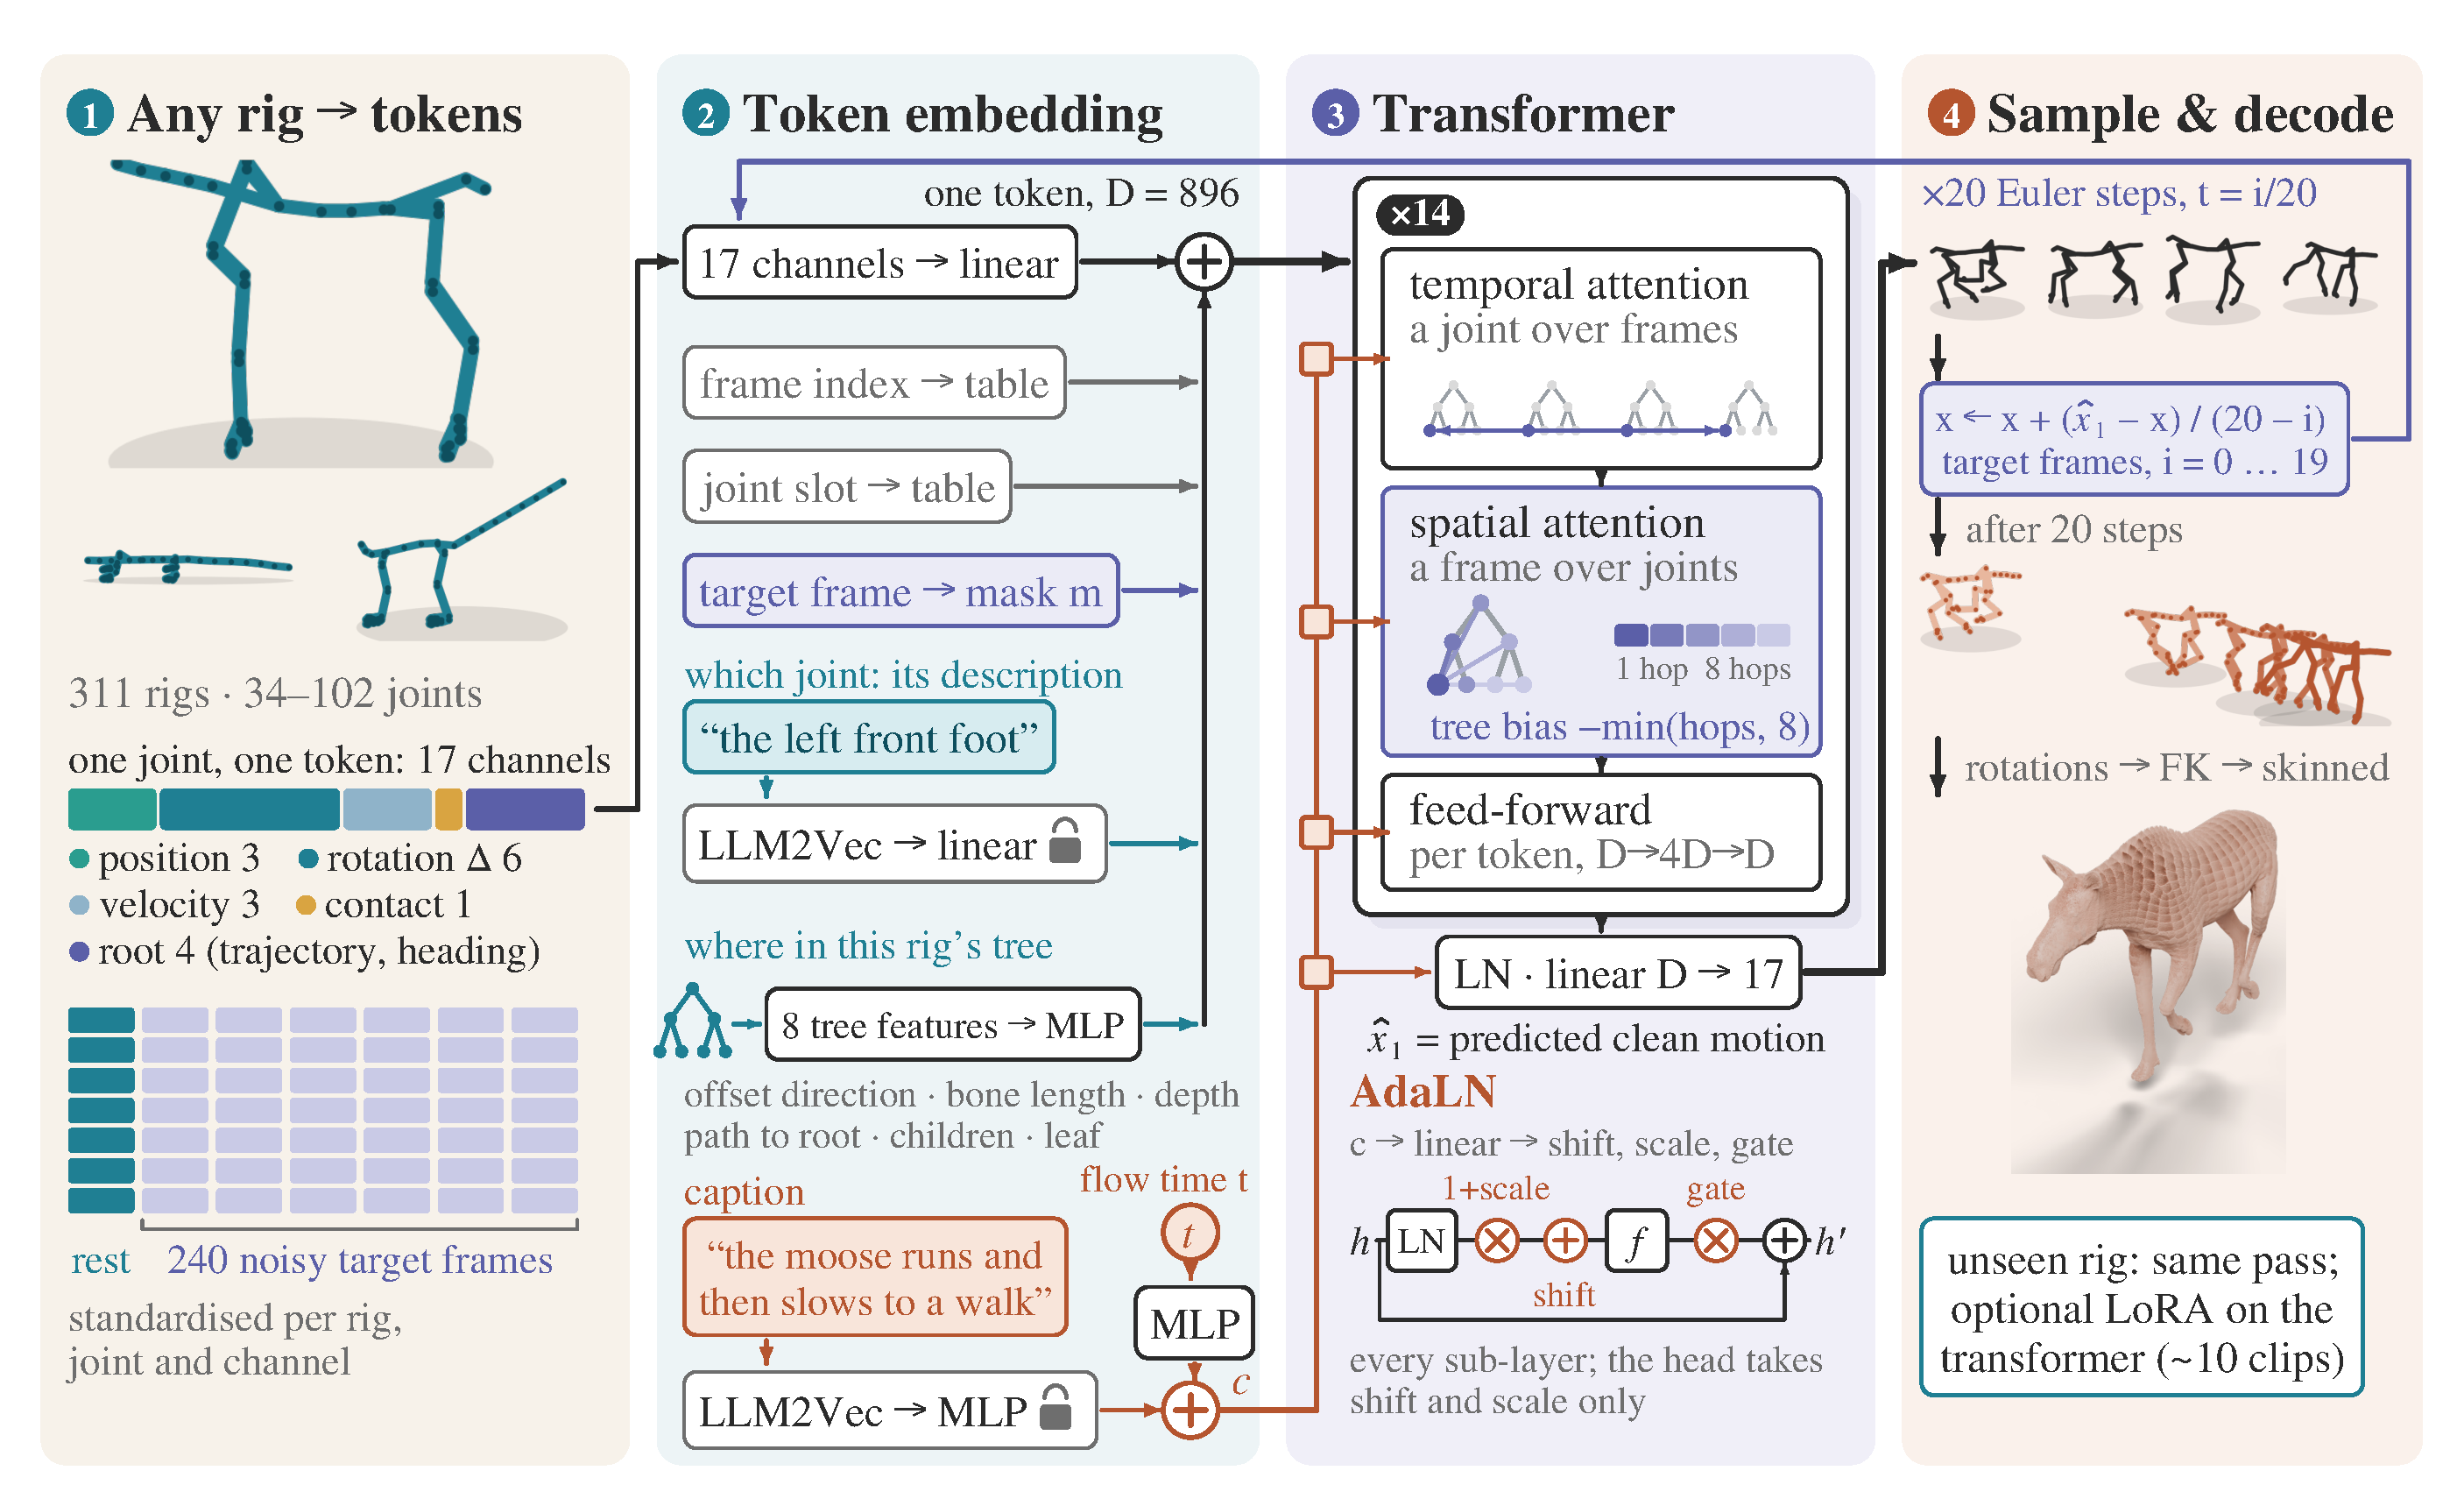
\includegraphics[width=\linewidth]{figures/fig1_align/figure1.pdf}
\caption{\method{} overview. A rig enters as data: one token per joint and frame with 17 standardised
channels, and the sequence is the rig's clean rest pose followed by the noise-mixed target frames. The
skeleton enters through the token sum (panel~2) and a tree-distance bias on spatial attention; the caption
and the flow time modulate every block through AdaLN. The head predicts the clean motion, the Euler steps
update the target frames only, and the rotations are played on the rig. An unseen rig takes the same pass.
All skeleton drawings are the model's own output on a moose run-to-walk clip.}\label{fig:teaser}
\end{figure}

\paragraph{Why one model for many skeletons is hard.} Four things stand in the way. There is no common
tensor: rigs differ in joint count, joint order, naming and scale, so cross-skeleton work has either
\emph{retargeted} onto a canonical skeleton~\citep{villegas2018nkn,aberman2020skeleton,lee2023same}, which
degrades as morphology diverges, or fixed a template body plan, which excludes every other body. The network
has to be told what each joint of an unfamiliar tree is and how the joints relate, without a parameter per
skeleton. A loss summed over a batch of rigs with 34 to 102 joints lets the largest bodies dominate, and
training such a model at 0.3B parameters is unstable without care. And a rig outside the training library has
to be served with no clips, or a handful, because a model per character multiplies data and compute by the
size of the cast. Generation across skeletons has been shown without text by AnyTop~\citep{gat2025anytop} on
the Truebones zoo, and with text by OmniZoo~\citep{chen2025omnizoo} on 140 species and by
G-MDM~\citep{lee2025dragon} on Truebones with joint rotations but no root translation.

\paragraph{Our position.} A generative model should treat the skeleton as \emph{input}, not as
architecture: told the kinematic tree, the rest pose and what each joint is, the network needs no
per-skeleton parameter, and adding a character becomes a data question. We study text-conditioned
generation of joint rotations and root trajectories across \num{311} production rigs at 0.3B parameters, on a
corpus that is a faithful sample of studio reality: \num{311} animal rigs with \num{34} to \num{102}
deformation joints (median 64), \num{108} distinct kinematic trees and \num{77{,}894} captioned clips
(\num{6.2}M frames).\footnote{The clips and their captions follow the AniMo4D annotation set of
\citet{wang2025animo}; the rigs are re-exported with deformation bones only, the joint descriptions are ours,
and the conversion to \rep{} is new (App.~\ref{app:rep}). The Truebones zoo, a publicly distributed set of 66
animal rigs, is kept entirely outside training.} The output is what a rig plays, per-joint rotations and a
world-space root trajectory, with no inverse-kinematics fit.

\paragraph{Contributions.}
\begin{enumerate}[leftmargin=*,itemsep=1pt,topsep=2pt]
\item \textbf{One text-to-motion system for hundreds of production skeletons, at 0.3B parameters}
  (\S\ref{sec:exp:main}). A single network trained on \num{311} rigs generates text-conditioned motion for
  every one of them and returns what the rig plays---rotations and a world-space root trajectory, no
  inverse-kinematics fit. The recipe trains a \num{303}M model stably, and retrieval and FID improve
  monotonically from \num{36}M to \num{303}M parameters.
\item \textbf{\rep{}, a motion representation designed so that any rigged animation becomes training data}
  (\S\ref{sec:method:rep}). A clip is converted from its kinematic tree, rest pose and motion alone---no
  template, retargeting, tokeniser or inverse kinematics---and every (rig, joint, channel) cell is
  standardised by its own statistics, which is what lets rigs of very different proportions share one
  network: 1.7--2.0 points of R@1 over a per-rig scale.
\item \textbf{Skeleton awareness inside the model: a rest-pose prompt and graph-biased attention}
  (\S\ref{sec:method:model}). The rig's clean rest pose leads the token sequence, and a tree-distance bias
  with learned ancestor tables lets spatial attention tell parent from child and one limb from another.
  Nothing in the network is indexed by rig, so a new rig is a new input; the flat padded-joint construction
  that fixed-skeleton generators are usually brought to variable skeletons with trails this design by
  0.19--0.20 of R@1.
\item \textbf{High fidelity in the library and zero- and few-shot generalisation outside it}
  (\S\ref{sec:exp:extend}). \method{} reaches R@1 \num{0.867} against \num{0.904} for the real clips and
  FID \num{0.005}. A rig the model has never seen is served by the same forward pass, and a low-rank adapter
  on roughly ten clips brings its rotation and position channels into agreement on bodies far from the
  training distribution (a winged dragon: from \num{4.46} to \num{0.30} bone lengths).
\end{enumerate}

\section{Related Work}\label{sec:related}

\paragraph{Text-to-motion generation.} Human text-to-motion has moved from VAEs on
HumanML3D~\citep{guo2022generating} to diffusion in pose space~\citep{tevet2023mdm,zhang2024motiondiffuse}
or a latent~\citep{chen2023mld}, distilled for real time~\citep{dai2024motionlcm}, and to token
models over a VQ-VAE~\citep{zhang2023t2mgpt,guo2024momask}, scaled by larger
corpora~\citep{lin2023motionx,fan2025motionmillion} and skeleton-aware latent
attention~\citep{hong2025salad}. All fix one kinematic tree; \method{} keeps the pose-space
diffusion and text conditioning and removes the fixed skeleton.

\paragraph{Motion across skeleton topologies.} Cross-skeleton motion has mostly meant
\emph{retargeting} between two known rigs~\citep{villegas2018nkn,aberman2020skeleton} or
skeleton-agnostic embeddings such as SAME~\citep{lee2023same} and SATA~\citep{zhang2026sata}, whose
text-conditioned generation is a downstream demonstration on HumanML3D. For generation on arbitrary
topologies, SinMDM~\citep{raab2024sinmdm} fits one motion at a time; AnyTop~\citep{gat2025anytop}
generates, without text, across the skeletons of the Truebones zoo~\citep{truebones}; UniMoGen~\citep{khani2025unimogen} is skeleton-agnostic and controlled by
style and trajectory. Text-conditioned animal motion has been approached from a fixed 35-joint
SMAL template by OmniMotionGPT~\citep{yang2024omnimotiongpt}, from a shared human--animal topology
by X-MoGen~\citep{wang2025xmogen} (115 species), across topologies by OmniZoo~\citep{chen2025omnizoo}
(a topology-aware skeleton embedding and 140 species), on a unified 30-joint skeleton by AniMo~\citep{wang2025animo}, whose AniMo4D
captions our corpus carries, on user-defined human skeletons by OmniSkel~\citep{liu2025omniskel},
on re-captioned Truebones data by G-MDM~\citep{lee2025dragon},
which generates Euler joint rotations without root translation, and, concurrently with this work, by
SAMoR~\citep{samor2026}, which pools any skeleton into eight part tokens over joint positions and
velocities and recovers rotations by inverse kinematics, and by UniMate~\citep{mou2026unimate}. \method{} is text-conditioned; it
denoises a per-joint representation any rig is converted to without a template, retargeting or inverse
kinematics; it embeds natural-language \emph{descriptions} of the joints with LLM2Vec; and it normalises
every (rig, joint, channel) cell with its own statistics, so that
hundreds of rigs of very different proportions share one network.

\paragraph{Objective, encoders, adaptation and evaluation.} \method{} is a DiT-style
denoiser~\citep{peebles2023dit} trained with flow matching~\citep{lipman2023flow,liu2023rectified},
classifier-free guidance on the text stream~\citep{ho2022cfg} and query--key
normalisation~\citep{dehghani2023vit22b}; its grouped per-channel-family objective follows
Kimodo~\citep{rempe2026kimodo}. Captions and joint descriptions are embedded with
LLM2Vec~\citep{behnamghader2024llm2vec} rather than CLIP~\citep{radford2021clip} or
T5~\citep{raffel2020t5}. New rigs are handled zero-shot through the skeleton prompt, in the spirit of
in-context conditioning for image diffusion~\citep{wang2023promptdiffusion}, and with a per-rig
LoRA~\citep{hu2022lora} when they lie far from the library. Retrieval metrics follow the contrastive text--motion evaluators
of~\citet{guo2022generating} and TMR~\citep{petrovich2023tmr}, which are tied to one skeleton; ours
is skeleton-aware (\S\ref{sec:method:eval}).

\section{Method}\label{sec:method}

A rig $\mathcal{R}=(\mathcal{T},\mathbf{p}^{\mathrm{rest}},\mathcal{D})$ is a kinematic tree
$\mathcal{T}$ over $J$ joints, a rest pose $\mathbf{p}^{\mathrm{rest}}\in\mathbb{R}^{J\times3}$ and
a natural-language description $\mathcal{D}=\{d_j\}_{j=1}^{J}$ of its joints. A motion is a tensor
$\mathbf{x}\in\mathbb{R}^{L\times J\times 17}$ in the \rep{} representation of
\S\ref{sec:method:rep}. Given $\mathcal{R}$ and a caption $c$, \method{} samples
$\mathbf{x}\sim p_\theta(\mathbf{x}\mid\mathcal{R},c)$ with one transformer shared by every rig
(\S\ref{sec:method:model}), trained by a calibrated grouped flow-matching objective
(\S\ref{sec:method:objective}) and sampled in 20 Euler steps
(\S\ref{sec:method:sampling}). A rig outside the training library is served by the same
forward pass and, when a few clips are available, by a per-rig LoRA
(\S\ref{sec:method:lora}); all retrieval metrics come from a skeleton-aware evaluator
(\S\ref{sec:method:eval}).

\subsection{\rep{}: a per-joint representation for any rig}\label{sec:method:rep}

\paragraph{Channels.} Every joint carries the same 17 channels (Table~\ref{tab:channels} in App.~\ref{app:rep}). Positions
are expressed relative to the root's own ground-plane track, with height absolute, so
that the body's pose and its travel are separated the way animators separate them. Rotations are
continuous 6D~\citep{zhou2019continuity} \emph{deltas} from the joint's rest orientation in the global
frame: ``no motion'' is the identity rotation, $[1,0,0,0,1,0]$ before normalisation, on every rig,
so that the rest frame means the same thing on every rig when it serves as the skeleton prompt
(\S\ref{sec:method:model}). Velocities are supervision only and are never
integrated at decode time, and the root comes from the trajectory channels. Every frame therefore decodes on its
own, without accumulated drift, by either of two routes that do not read each other: the position channels, or
forward kinematics from the rotation channels. Their disagreement is the FK--pose gap this paper reports --- a property
the representation exposes, not a metric imposed on it. Everything is expressed in one canonical frame ($+Y$ up, rest forward $+Z$) obtained
by a rigid per-rig re-alignment to the foot support plane, after which forward kinematics is
unchanged to numerical precision (App.~\ref{app:rep}). Building \rep{} for a new rig needs only its
kinematic tree, rest pose and animation: there is no template skeleton, no retargeting and no
inverse-kinematics fitting, and the same channel definition converts every
Truebones rig used in \S\ref{sec:method:lora}.

\paragraph{Per-cell normalisation.} Rigs differ in size, proportion and convention by orders of
magnitude, so every (rig, joint, channel) cell is standardised with its own mean and standard
deviation, the latter floored at $\epsilon_\sigma$ (\S\ref{sec:exp:setup}), and cells that are constant across
a rig's library, such as never-firing contact flags, are removed from supervision (App.~\ref{app:rep}). The
statistics are a property of the rig, computed from its motion library and supplied with it at deployment,
just as motion-transfer tools require example motions of the target
character~\citep{chen2025motion2motion}. The library, its split and the conversion are described in
\S\ref{sec:exp:setup} and App.~\ref{app:rep}.

\subsection{In-context skeleton conditioning}\label{sec:method:model}

\paragraph{Tokens and layout.} One token per frame and joint (Figure~\ref{fig:teaser}, \emph{any rig
$\to$ tokens}): the 17 channels of a cell are projected to width $D$ and receive a frame-index and a
joint-slot embedding. The sequence is $[\,\mathbf{x}^{\mathrm{demo}}\mid\mathbf{x}_t^{\mathrm{tgt}}\,]$
along time: one clean frame holding the rig's analytic rest pose, never noised, followed by the $L$
target frames (\S\ref{sec:exp:setup}), which carry the flow interpolant and a learned marker and are the
only frames denoised and scored. Under the rest-delta parameterisation the rest frame's rotations are the identity
on every rig, so it conveys proportions, joint count and graph rather than motion; after per-cell
normalisation it also carries the rig's statistics.

\paragraph{Three signals identify the skeleton.} Nothing in the network is indexed by rig; what it knows
about a body arrives as input (Figure~\ref{fig:teaser}, \emph{token embedding}). \emph{Geometry}: the
rest frame above. \emph{Identity}: each joint description $d_j$ is embedded once with frozen
LLM2Vec~\citep{behnamghader2024llm2vec} (4096-d), projected and added to every token of joint $j$.
We use descriptions rather than bone names because ``front left upper leg'' is the same concept on a horse
and a lizard whereas \texttt{L\_Femur\_02} and \texttt{b\_hindleg\_l\_1} are not, and a new rig's
naming scheme need never have been seen. \emph{Place in the tree}: an 8-d structural vector per joint
(rest-offset direction, bone length, tree depth, root-path length, child count, leaf flag) passes
through a zero-initialised MLP and is added to the same tokens.

\paragraph{The graph enters as an attention bias.} Each of the $N_b$ blocks factorises attention over the
two token axes (Figure~\ref{fig:teaser}, \emph{transformer}): temporal attention, one joint over its
frames; spatial attention, one frame over its joints; then a $4\times$ MLP. Only the spatial attention
sees the kinematic tree, as an additive per-head bias on the logits between joints $i$ and $j$,
$b^{(h)}_{ij}=-g_{ij}+u^{(h)}_{a_{ij}}+d^{(h)}_{s_{ij}}$, where $g_{ij}$ is the hop distance on the tree,
clipped at $g_{\max}$, $a_{ij},s_{ij}$ are the hops up and down to the lowest common ancestor, clipped at
$a_{\max}$ (\S\ref{sec:exp:setup}), and $u,d$ are zero-initialised per-head tables. Nearer joints attend
more by default, and the tables let a head tell parent from child, and a joint on the same limb from one
across the body (App.~\ref{app:model}). The
tree is a soft prior on a fully connected joint attention, not a fixed layer, so one network serves
any joint count and topology.

\paragraph{Text and time modulate.} The conditioning vector
$\mathbf{c}=\mathrm{MLP}(t)+\mathrm{MLP}(\mathbf{e}_c)$, with $\mathbf{e}_c$ the pooled LLM2Vec caption
embedding, drives the AdaLN~\citep{peebles2023dit} shift, scale and gate of every sub-layer (shift and scale
only on the output head), so text reaches the model only through modulation and the token stream stays
kinematic. The caption is dropped with probability $p_{\mathrm{drop}}$ (\S\ref{sec:exp:setup}) for
classifier-free guidance; the rest-pose prompt is never dropped.

\paragraph{Stability.} Queries and keys are RMS-normalised per head before the dot
product~\citep{dehghani2023vit22b}; without it, every attempt at 0.3B diverged (App.~\ref{app:ablation_notes}).

\subsection{Calibrated grouped flow-matching objective}\label{sec:method:objective}

\paragraph{Flow matching with $\mathbf{x}$-prediction.} We train on the straight path
$\mathbf{x}_t=(1-t)\,\mathbf{x}_0+t\,\mathbf{x}_1$ with $\mathbf{x}_0\sim\mathcal{N}(0,I)$ and
$t\sim\mathcal{U}(0,1)$~\citep{lipman2023flow,liu2023rectified}; the network predicts the clean
sample $\hat{\mathbf{x}}_1$, and the velocity-space weight of \citet{li2025jit} is applied,
\begin{equation}
  \ell(\mathbf{x}_t,t)=\frac{w(t)}{\mathbb{E}[w]}\;\mathrm{Huber}_{\delta}\!\left(\hat{\mathbf{x}}_1-\mathbf{x}_1\right),
  \qquad w(t)=\frac{1}{\max(1-t,\,\sigma_{\min})^{2}},
  \label{eq:elem}
\end{equation}
with $\mathrm{Huber}_{\delta}(r)=r^{2}$ for $|r|\le\delta$ and $\delta(2|r|-\delta)$ beyond, applied per cell;
$\delta$ sits below the 99.99th percentile of the normalised targets (App.~\ref{app:calib}), $\sigma_{\min}$
and $\delta$ are given in \S\ref{sec:exp:setup}, and $t$ is sampled uniformly (App.~\ref{app:ablation_notes}).

\paragraph{Grouped loss.} A rig with 102 joints has three times the body cells of one with 34 and
the same single root row, so a plain mean over cells would drown the root trajectory, heading and
contact channels---the ones that decide whether a walk is a walk---in body rotations on large rigs.
We partition the channels into nine groups $g$: position, rotation and velocity, each for the root and
for the body, plus contact, root track and heading, and use
\begin{equation}
  \mathcal{L}=\sum_{g}\gamma_g\sqrt{\frac{N_g}{N}}\;\bar{\ell}_g,
  \label{eq:grouped}
\end{equation}
where $\bar{\ell}_g$ is the masked mean of Eq.~(\ref{eq:elem}) over the $N_g$ valid cells of group
$g$ in the batch and $N=\sum_g N_g$; the $\gamma_g$ are set by the calibration below, following the
target-share weighting of Kimodo~\citep{rempe2026kimodo}.
Under this weighting the explicit $N_g$ dependence of the output-gradient energy of group $g$
cancels: it is proportional to $\gamma_g^{2}Q_g$, where $Q_g$ is the group's mean weighted squared
residual, so a group's weight in $\partial\mathcal{L}/\partial\hat{\mathbf{x}}_1$ no longer grows
with the number of cells the group spans in the batch (App.~\ref{app:calib}).

\paragraph{Calibration.} The $\gamma_g$ are not hand-tuned. A target share profile over channel
families is fixed in advance, the group energies $E_g$ are measured over one pass of the training set
under exactly the training crops and masks, and the weights are solved as
$\gamma=\sqrt{\text{share}/E}$, with the rotation family anchored at $\gamma_{\mathrm{rot}}$
(\S\ref{sec:exp:setup}) and the others solved relative to it. A \emph{mechanism check} then takes a few
optimiser-free steps of a small model of the same recipe and verifies that every family's measured share of
$\|\partial\mathcal{L}/\partial\hat{\mathbf{x}}_1\|^{2}$ matches the $\gamma_g^{2}Q_g$ prediction
(App.~\ref{app:calib}). It certifies the wiring of the weights, not that the profile fixed in advance is
realised during training: the realised share moves with the error energies, which evolve.

\paragraph{Auxiliary terms.} Four terms are added with weights $\lambda_{\mathrm{FK}}$,
$\lambda_{\mathrm{vel}}$, $\lambda_{\mathrm{lock}}$ and $\lambda_{\mathrm{acc}}$ (\S\ref{sec:exp:setup}), none
carrying the time weight $w(t)$: a forward-kinematics consistency term between predicted positions and
positions forward-kinematised from predicted rotations, a velocity term on world joint displacements, a
foot-lock term gated by the contact channel, and an acceleration-matching term (App.~\ref{app:calib}).

\subsection{Sampling}\label{sec:method:sampling}
Samples follow the straight path with Euler steps
$\mathbf{x}\leftarrow\mathbf{x}+(\hat{\mathbf{x}}_1-\mathbf{x})/(S-i)$ over $S$ steps; invalid cells are
projected back to zero after every step, and guidance is applied to the caption only,
$\hat{\mathbf{x}}_1=\hat{\mathbf{x}}_1^{\varnothing}+s\,(\hat{\mathbf{x}}_1^{c}-\hat{\mathbf{x}}_1^{\varnothing})$
with guidance scale $s$ (\S\ref{sec:exp:setup}). Twenty steps is the operating point used throughout; ten give the same retrieval at half the
cost, and App.~\ref{app:cost} gives the latency and quality of both.

\subsection{Extending the model to a rig it has never seen}\label{sec:method:lora}
\paragraph{Zero-training arm.} An unseen rig is served by the frozen backbone as soon as its rest
pose, joint descriptions and per-cell statistics (from its own clips) are supplied; on the Truebones
rigs this yields motion with far more jitter than the real clips, since wing chains and eight-legged
gaits are absent from the training prior.

\paragraph{Per-rig LoRA.} When roughly ten clips of the new rig exist, we attach rank-64 or rank-128
adapters~\citep{hu2022lora} (scale 1) to the attention projections, the MLPs and the conditioning
paths (joint-semantics projection, caption MLP, structural MLP, AdaLN), leaving the input and output
projections and the timestep MLP frozen; the adapters hold 26.8M (r64) or 53.6M (r128) parameters
and are folded back into the weights at export, so every consumer loads a plain checkpoint. The
new rig's data view is built by the corpus script (joint pruning to the deformation-bone convention,
corpus-style captions, an 80/20 split) and the adapter is trained with the backbone
recipe for 300--900 epochs (App.~\ref{app:lora}); a single adapter shared by a group of rigs
removes the same jitter excess on all of them, and matches a per-rig adapter on the one rig where both were
trained (App.~\ref{app:extend_more}).

\subsection{Skeleton-aware evaluation}\label{sec:method:eval}
\paragraph{Evaluator.} Retrieval metrics require a text--motion embedding, and existing ones are
tied to one skeleton. We train two towers into a shared 512-d space: a frozen DistilBERT text tower
with a trainable pooling head, and a graph-aware motion tower (6 graph layers, 4 temporal layers)
over the \rep{} channels without contact, with a symmetric InfoNCE objective. The
evaluator sees only real data, never generated samples, and shares no weights with the generator.

\paragraph{Protocol.} Text$\to$motion R@1/2/3 in pools of 64, matching score and FID in the
evaluator space, each next to the evaluator's score on the real clips of the same pools (with shuffled
captions the evaluator scores R@1 \num{0.035} in pools of 32, chance \num{0.031}); generation is fixed at 20 steps,
$s{=}2$ at seed 42 and sharded across GPUs under a hashed generation plan with provenance checks.
Rigs outside the library, for which no evaluator exists, are scored geometrically
(\S\ref{sec:exp:setup}).

\section{Experiments}\label{sec:exp}

We ask four questions. (1) How well does one set of weights serve hundreds of heterogeneous
skeletons on text-conditioned generation (\S\ref{sec:exp:main})? (2) How far does the model
extend to a rig it has never seen, with no training and with about ten clips
(\S\ref{sec:exp:extend})? (3) Which capabilities does it combine that released
systems provide separately, and what does the released arbitrary-topology model produce on the same rigs
(\S\ref{sec:exp:compare})? (4) Which ingredients matter
(\S\ref{sec:exp:ablation})?

\subsection{Setup}\label{sec:exp:setup}

\paragraph{Library and splits.} The training library is the \num{311}-rig animal corpus of
\S\ref{sec:method:rep} (\num{77{,}894} clips, \num{6.18}M frames at 30\,fps, 34--102 joints).
Validation holds \num{3{,}899} clips over \num{311} rigs (\num{5}\% of every rig's clips, drawn by a
one seeded permutation per rig; App.~\ref{app:split}). For rigs outside the library we use the
Truebones zoo~\citep{truebones}: \num{986} clips over \num{66} rigs after conversion to \rep{}
with the same pipeline (\num{802} of them carry a caption). Each Truebones rig is split
$80/20$ into train and validation clips by source animation, so that a clip and its cut
neighbours never straddle the split.

\paragraph{Models.} The main model has \num{303}M parameters (14 blocks, width 896, 14 heads);
a \num{36}M pilot (8 blocks, width 384, 6 heads) shares every other setting and is used for
ablations. Both train at global batch 128 with the calibrated objective, the main model for
\num{290} epochs at $1.5{\times}10^{-4}$ and the pilot for 400 at $2{\times}10^{-4}$, with a
4{,}000-step warm-up and a half-cosine decay over 40 epochs to $1\%$ of the peak.

\paragraph{Protocol.} Generation uses 20 Euler steps and text guidance $s{=}2$ everywhere
(\S\ref{sec:method:sampling}); each clip is generated at the length of the real clip, capped at
240 frames, with one seed. Retrieval metrics follow \S\ref{sec:method:eval}: text-to-motion
R-precision at $K{=}1,2,3$ in pools of 64 formed by chunking the dataset order (a retrieved motion
is correct if it is the caption's clip, another export of the same source motion, or a clip with an
identical caption), the FID on the evaluator's
$\ell_2$-normalised embeddings, and the text--motion matching score, each next to the evaluator's
score on the real clips of the same pools (a reference, not a bound). Because a skeleton-aware evaluator exists
only for the library rigs, the Truebones experiments are scored geometrically, in world space,
on the deployable output (the forward kinematics of the predicted rotations): the articulation ratio (mean joint speed relative to the root,
divided by the real clips' value), the jitter ratio (mean second temporal difference, likewise
normalised) and the root speed ratio. Ratios are taken against \emph{all} real clips of the rig at a common 20\,Hz, so that AnyTop samples
and ours are measured identically. The \emph{FK--pose gap} is the mean distance, in the rig's
mean bone length, between the joint positions obtained by forward kinematics of the predicted
rotations and the directly predicted ones: a consistency of the two channels, not a distance to the
target, read from the training-time validation pass (App.~\ref{app:calib}). Library clips are
generated at the real clip's length (at most 240 frames)
from the epoch-289 checkpoint with seed 42; the Truebones arms of \S\ref{sec:exp:extend} use the
epoch-214 snapshot that initialised the adapters, seed 7.

\subsection{One model for 311 skeletons}\label{sec:exp:main}

Table~\ref{tab:main} reports text-to-motion retrieval on the validation set. All \num{311} rigs appear in
training, so this measures the generation of held-out clips on known rigs; rigs outside the library are
the subject of \S\ref{sec:exp:extend}. The \num{303}M
model reaches R@1 \num{0.922} against \num{0.964} for the real clips scored by the same evaluator
in the same pools, a text--motion matching score of \num{0.764} against \num{0.782}, and an FID of
\num{0.005}; the \num{36}M pilot, trained on the same data with the same recipe, reaches R@1
\num{0.897} and FID \num{0.008}. The pools follow the dataset order, so a pool holds clips of one
rig or of neighbouring rigs; R-precision uses the \num{3{,}840} clips of the 60 complete pools, the
matching score and the FID all \num{3{,}899}. The 95\% bootstrap interval over pools is
$[\num{0.907}, \num{0.936}]$ for the \num{303}M R@1 and $[\num{0.955}, \num{0.971}]$ for the real
clips (App.~\ref{app:controls}).

\begin{table}[t]
\centering\small
\caption{Text-to-motion generation on the validation set (\num{3{,}899} clips over \num{311} rigs; 60 pools
of 64, 20 steps, $s{=}2$, one seed; Table~\ref{tab:pool} gives the other pool sizes). The reference row scores the
real clips with the same evaluator in the same pools. R-precision is text$\rightarrow$motion; Match is the mean
text--motion cosine; FID is on the evaluator's normalised embeddings.}\label{tab:main}
\begin{tabular}{lcccccc}
\toprule
& Params & R@1$\uparrow$ & R@2$\uparrow$ & R@3$\uparrow$ & FID$\downarrow$ & Matching$\uparrow$ \\
\midrule
Real clips (reference) & -- & \num{0.964} & \num{0.998} & \num{0.999} & 0 & \num{0.782} \\
\method{} (pilot) & \num{36}M & \num{0.897} & \num{0.966} & \num{0.982} & \num{0.008} & \num{0.746} \\
\method{} & \num{303}M & \num{0.922} & \num{0.982} & \num{0.992} & \num{0.005} & \num{0.764} \\
\bottomrule
\end{tabular}
\end{table}

\paragraph{What the score responds to.} Five controls (App.~\ref{app:controls}) locate the
\num{303}M model's R@1 of \num{0.922}. Re-deriving its joint positions from its own rotations leaves
\num{0.923}; permuting its frames leaves \num{0.805}. Two degenerate sequences built from real data
set the floor: the target clip's own first pose, held for its duration, scores \num{0.346}, and the
rig's rest pose \num{0.109}, against a chance level of \num{0.018}. Giving every clip in a pool
another clip's caption leaves \num{0.005}. A static pose of the right species is therefore already worth
\num{0.346} under this protocol. Table~\ref{tab:controls} gives the same controls for the pilot and the two
representation arms, and Figure~\ref{fig:qual} shows seven generated clips on the rigs' production meshes.

\begin{figure}[t]
\centering
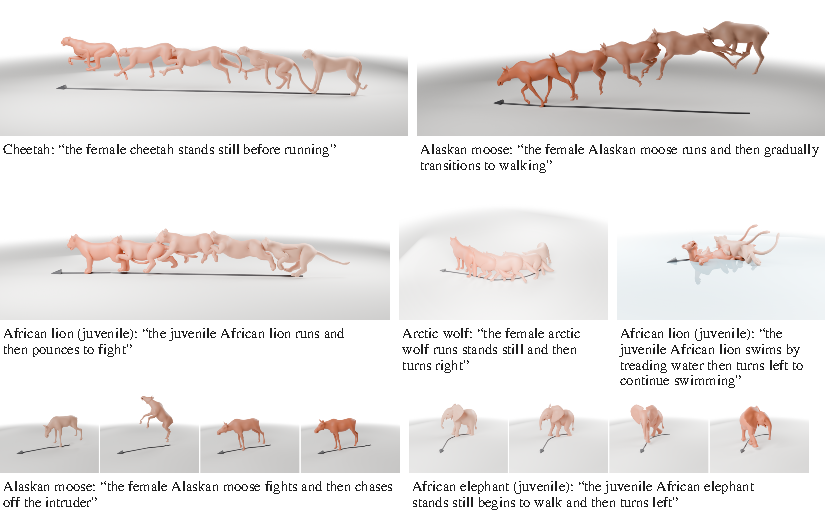
\includegraphics[width=0.9\linewidth]{figures/qualitative.pdf}
\caption{Seven generated clips of five library rigs on their production meshes. Travelling actions: four to
five poses at equal distances along the root path, light (first) to dark (last), with the root trajectory on the
ground. Actions on the spot: four frames at equal times from a fixed camera. Captions are the clips'
own.}\label{fig:qual}
\end{figure}

\subsection{Extending the model to rigs it has never seen}\label{sec:exp:extend}

\paragraph{Zero training and per-rig LoRA.} We take four Truebones rigs that differ from the
library in body plan and joint count -- Buffalo (30 joints), Gazelle (29), Dragon (95 joints, a
flying rig) and Spider (68) -- and compare three arms on the same held-out clips of each rig:
(a) the library model with the new rig's per-cell statistics, computed from all of its clips including
the evaluation clips, as its only rig-specific input (\emph{zero training}); (b) a per-rig
low-rank adapter trained on the rig's 8--26 training clips (\emph{LoRA}, \S\ref{sec:method:lora});
(c) a \num{36}M model of the same recipe trained on all \num{802} captioned Truebones clips,
evaluation clips included, as a seen-clip reference.
Table~\ref{tab:lora} gives the FK--pose gap on the held-out clips before and after adaptation next
to the articulation and jitter of the sampled output: eight to twenty-six clips bring the gap from
$0.25$--$1.2$ bone lengths to $0.08$--$0.15$, most on the two rigs farthest from the library, and
the seen-clip reference sits at $0.06$--$0.13$. Most of that is bought early: the jitter of the zero-training arm is
gone within 50--100 epochs and the gap plateaus by 150--200, after which longer adaptation changes nothing
(App.~\ref{app:extend_more}).

\begin{table}[t]
\centering\footnotesize\setlength{\tabcolsep}{3.5pt}
\caption{Extending \method{} (\num{303}M) to four Truebones rigs, each arriving with its own per-cell
statistics and masks. \emph{zero}: the library model served with those statistics and nothing
else --- articulation and jitter from that model, the gap from the adapter run's first validation, 10 to 15
steps in; \emph{LoRA}: the per-rig adapter; \emph{TB-only}: a \num{36}M model trained on all Truebones clips
including these. Gap in bone lengths; articulation and jitter of the sampled FK output relative to all real
clips of the rig (1 = real). App.~\ref{app:lora} and App.~\ref{app:extend_more} give the settings, the
\num{36}M study and a shared adapter for eight flying rigs.}\label{tab:lora}
\begin{tabular}{@{}llccccccccc@{}}
\toprule
& & \multicolumn{3}{c}{FK--pose gap (bl)$\downarrow$} & \multicolumn{3}{c}{Articulation ratio} & \multicolumn{3}{c}{Jitter ratio} \\
\cmidrule(lr){3-5}\cmidrule(lr){6-8}\cmidrule(lr){9-11}
Rig & Train / val & zero & LoRA & TB-only & zero & LoRA & TB-only & zero & LoRA & TB-only \\
\midrule
Buffalo (30 j.) & 15 / 5 & \num{0.323} & \num{0.132} & \num{0.072} & \num{1.45} & \num{0.30} & \num{0.67} & \num{3.32} & \num{0.33} & \num{1.02} \\
Gazelle (29 j.) & 8 / 2  & \num{0.255} & \num{0.084} & \num{0.062} & \num{5.39} & \num{0.77} & \num{1.22} & \num{13.2} & \num{0.86} & \num{1.92} \\
Dragon (95 j.)  & 10 / 3 & \num{1.215} & \num{0.146} & \num{0.134} & \num{1.02} & \num{0.49} & \num{1.23} & \num{2.53} & \num{0.52} & \num{1.12} \\
Spider (68 j.)  & 26 / 6 & \num{1.029} & \num{0.130} & \num{0.088} & \num{2.87} & \num{0.24} & \num{0.35} & \num{6.49} & \num{0.20} & \num{0.37} \\
\bottomrule
\end{tabular}
\end{table}

\subsection{Relation to prior work}\label{sec:exp:compare}

\paragraph{Capabilities.} The two capabilities this paper joins are available separately in released
systems (Table~\ref{tab:open}): those that take the kinematic tree at inference are not text-conditioned, and
the text-conditioned animal generators are built around one fixed skeleton. \method{} returns rotations and a
world-space root trajectory the rig plays as generated, and measures that geometry against ground truth for the
pilot and the main model alike (Table~\ref{tab:physical}: at \num{303}M the FK--pose gap is \num{0.24} bone
lengths, the foot slide \num{1.84} against a real \num{2.03}). Table~\ref{tab:capability} adds the systems whose
code is not public. The construction those systems reach a second skeleton with --- every joint padded into one
flat per-frame vector --- is trained on our corpus at our budget in App.~\ref{app:flat} and read beside the
ablations in Table~\ref{tab:simple}.

\begin{table}[t]
\centering\footnotesize\setlength{\tabcolsep}{4pt}
\caption{Systems with a public implementation we could run. \emph{Topology}: the kinematic tree is an input at
inference, not fixed by the architecture. \emph{Rotations} / \emph{Root}: joint rotations and a world-space root
trajectory, not positions a solver must turn back into a pose.}\label{tab:open}
\begin{tabular}{@{}lccccc@{}}
\toprule
System & Code & Text & Topology & Rotations & Root \\
\midrule
Human T2M~\citep{tevet2023mdm,zhang2024motiondiffuse} & $\checkmark$ & $\checkmark$ & $\times$ & $\checkmark$ & $\checkmark$ \\
Animal T2M~\citep{wang2025animo,yang2024omnimotiongpt} & $\checkmark$ & $\checkmark$ & $\times$ & $\checkmark$ & $\checkmark$ \\
AnyTop~\citep{gat2025anytop} & $\checkmark$ & $\times$ & $\checkmark$ & $\checkmark$ & $\checkmark$ \\
\method{} (ours) & --- & $\checkmark$ & $\checkmark$ & $\checkmark$ & $\checkmark$ \\
\bottomrule
\end{tabular}
\end{table}


\paragraph{AnyTop as an in-distribution reference.} The released AnyTop weights trained on the whole
Truebones zoo, including the four rigs of Table~\ref{tab:lora}, so its per-rig geometry
(App.~\ref{app:anytop}) is a reference for what a model trained on these rigs produces.

\subsection{Ablations}\label{sec:exp:ablation}

The ablations share the pilot's recipe and checkpoint epoch; App.~\ref{app:ablation_notes} collects them
with the notes. Flattening the joint axis into one token per frame --- the construction that carries a
fixed-skeleton generator to variable skeletons --- costs \num{0.198}--\num{0.208} of R@1 and multiplies the FID
by \num{3.7}, with the corpus, split, captions, rest pose, objective, weights, schedule and budget matched and
\num{5}\% more parameters on the flat side (Table~\ref{tab:simple}, App.~\ref{app:flat}). Keeping the joint
axis and removing what this paper puts on it costs \num{0.067}--\num{0.072}, of which the calibrated group
weights carry \num{0.036}--\num{0.045}, the geodesic and direction biases and the structural features
\num{0.028}--\num{0.035}, and the joint descriptions none. The acceleration-matching
term changes nothing (Table~\ref{tab:ablation}). Per-cell mean and standard deviation are worth about two points of R@1 over a per-rig scale alone and \num{22}--\num{30}\% of the FID at every matched
epoch (Table~\ref{tab:rep}). Its channel layout is worth under a point of R@1 against the 13-channel AnyTop
layout derived from the same clips (Table~\ref{tab:repcontent}), and \num{0.007} once that arm's own objective
and partition are matched, so retrieval is measuring the objective rather than the layout; what the layout does
change is the leaf articulation, foot contact and root travel of Table~\ref{tab:physical}, and the agreement of
the two output channels --- re-encoding a sample through the forward kinematics of its own rotations costs
\num{0.005} of R@1 on \rep{} against \num{0.035} on the 13-channel layout (Table~\ref{tab:controls}). At a
matched budget of 200 epochs the \num{36}M, \num{116}M and \num{303}M models reach R@1 \num{0.878},
\num{0.900} and \num{0.914} (Table~\ref{tab:size}).


\section{Conclusion}\label{sec:conclusion}

A text-to-motion model can treat the skeleton as an input rather than as part of the architecture:
one \num{303}M-parameter model trained on \num{311} animal rigs generates text-conditioned motion for
all of them (R@1 \num{0.864} against \num{0.904} for the real clips), returning rotations and a root
trajectory the rig plays directly, and a low-rank adapter on eight to twenty-six clips extends it to
rigs outside the library. The library is animal-only, and the extension study covers four rigs.

\section*{Reproducibility statement}

Section~\ref{sec:method:rep} and Appendix~\ref{app:rep} specify the representation channel by
channel, the conversion from a kinematic tree, rest pose and motion, and the per-cell
normalisation; Appendix~\ref{app:calib} gives the calibration protocol, the target share profile
and the mechanism check that certifies an artifact; Appendix~\ref{app:lora} lists every adapter
hyper-parameter; Appendix~\ref{app:flat} gives the adapted baseline's construction and everything it is
given; Appendix~\ref{app:anytop} gives the AnyTop sampling protocol and the geometric
protocol, including the frame-rate handling. All evaluation runs are seeded, and the sharded
generation used for retrieval metrics records the checkpoint, sampler and source hashes so that
a table can be re-scored from the stored samples.

\subsection*{AI use statement}
We used generative AI tools throughout this work. The code for data conversion, training, evaluation
and rendering was drafted with an LLM-based coding assistant and independently reviewed by a second
LLM reviewer before it was run; every script was tested, and every number in this paper was checked
against the run logs and artifacts by the authors. LLM assistance was also used for experiment
orchestration, for auditing the data, for figure scripts, literature search
and the drafting and editing of the text. The joint descriptions were produced with an LLM from the joint names; the clip captions are the
AniMo4D annotations~\citep{wang2025animo}. The research
questions, the design decisions and the interpretation of the results are the authors', and we take
responsibility for the final content, including text, claims and artifacts produced with the aid of
generative AI.

\subsection*{Ethics statement}
The work involves no human subjects and no personal data. The training library follows the clip
inventory and captions of AniMo4D~\citep{wang2025animo}, and the evaluation rigs come from the publicly
distributed Truebones zoo. The paper specifies the conversion channel by channel, so the representation
can be rebuilt from the same sources. Generated animal motion for games and film carries no risk beyond
the generic misuse of animation tools.


\bibliography{references}
\bibliographystyle{iclr2027_conference}

\newpage
\appendix

\section{\rep{} details}\label{app:rep}

\begin{table}[t]
\centering\small
\caption{\rep{} channel layout per joint and frame. Channels 13--16 exist on the root row only; every
(rig, joint, channel) cell is normalised with its own statistics and exactly-constant cells are
excluded from supervision.}
\label{tab:channels}
\begin{tabular}{@{}llll@{}}
\toprule
slice & content & frame & supervised on \\
\midrule
0:3   & position (XZ relative to the root track, Y absolute) & world & all joints \\
3:9   & rotation, continuous 6D delta from the rest orientation & global & free-DOF joints \\
9:12  & world velocity (supervision only, never integrated) & world & all joints \\
12    & contact flag & --- & joints with contact \\
13:15 & root trajectory XZ & world & root only \\
15:17 & heading $(\cos\phi,\sin\phi)$ & world & root only, valid frames \\
\bottomrule
\end{tabular}
\end{table}


\paragraph{Validity.} Not every cell exists on every rig or frame. Frame and joint masks handle
padding; rotation is supervised only on joints with free degrees of freedom, contact only on joints
that can touch the ground, heading only on frames where it is defined. The per-rig cell mask
multiplies the interpolant, the loss and the per-step projection at sampling time, so an invalid cell
is exactly zero everywhere rather than ``small''. Per-frame heading validity is the one part of the
mask that training has and sampling does not: it gates the target's heading channels during training,
while at generation the target's heading is what is being generated, so the sampler carries the
demonstration's flag only and the target heading is produced unconditionally.


\paragraph{Why standardise rather than scale.} We found this to be decisive. Under the scale-only
normalisation of the source protocol a large part of the objective is already explained by a constant
pose, and the network settled on a frozen pose while the root travelled. On a 671-window probe of an
earlier build, a constant prediction recovers $75\%$ of the scale-only objective; centring each cell
on its mean brings that to $41.6\%$, and centring and dividing by the standard deviation, the
normalisation used here, brings it lower still. Table~\ref{tab:rep} measures the consequence directly on
the corpus used here: at every matched epoch the standardised representation is about two points of
R@1 ahead, with the FID \num{22}--\num{30}\% lower. 

\paragraph{Conversion.} A clip enters as a kinematic tree, a rest pose and per-frame local
rotations and root translation. It is first resampled to 30\,fps (linear interpolation of the root
translation, spherical interpolation of the local rotations, then forward kinematics) and expressed
in a right-handed canonical basis. Global joint rotations follow from forward kinematics; the
\emph{heading} is the ground-plane direction between a designated pair of joints of the rig,
stored as the unit vector $(f_z, f_x)$ and marked invalid (channels set to zero, excluded from
supervision) on frames where that projected direction has length below $10^{-6}$. The \emph{root
track} is the root joint's own XZ trajectory, stored unsmoothed on the root row; joint positions store
XZ relative to it and Y as absolute height, so every window can be re-based to its own first frame
without touching the pose. Rotations are the global rotation composed with the inverse rest rotation of the same joint,
encoded as the first two matrix columns (continuous 6-D), so a joint at rest is the identity on every
rig. Velocities are one-step finite differences of world positions, per second, supervised but never
integrated. A contact flag marks the frames on which a joint that can touch the ground is within
$0.3$ of the lowest point its rig's contact joints reach in the clip and whose squared displacement to
the next frame is at most $0.002$ (canonical units; both tests read the following frame, so the flag
at frame $t$ describes the step from $t$ to $t{+}1$). The Truebones corpus was converted by an earlier
build of the same codec, which smoothed the root track with a $1$\,Hz zero-phase filter, took the
heading from the carrier joint's rotation with a $0.05$ validity floor, and set contact from
normalised height and speed ($0.05$ and $0.25$); the main-body pruning of Appendix~\ref{app:lora}
precedes it. Both builds write the same 17 channels with the same meanings, which is what lets one
model serve a rig from either corpus, and every Truebones number here is measured within that corpus.

\paragraph{Per-cell statistics.} For every rig, joint and channel the mean and standard deviation
are taken over all frames of all of the rig's clips (heading channels over valid frames only), and a
cell is served as $(x-\mu)/(\sigma+10^{-6})$ with $\sigma$ raised to at least $0.05$. A cell whose
value never changes on a rig (contact of a joint that never touches the ground, a fixed degree of
freedom) is exactly constant; it is normalised to zero, excluded from supervision and held at its
constant when decoding. On the library this concerns $9{,}185$ of the $256{,}512$ cells that exist
on the \num{311} rigs, \num{9{,}123} of them contact flags. A rig outside the
library is served the same way from statistics computed on its own clips; how far a rig can be served
without them is the subject of \S\ref{sec:exp:extend}.

\paragraph{Corpus statistics.} The library holds \num{311} rigs and \num{77{,}894} clips
(\num{73{,}995} training, \num{3{,}899} validation), \num{6.18}M frames at 30\,fps, or $57$
hours. Clips are short: median $62$ frames, mean $79$, maximum $299$, and $2.1\%$ exceed the
240-frame training window. Rigs have between $64$ and $946$ clips (median $236$). Joint counts run from
$34$ to $102$ (median $64$): $61$ rigs in the thirties, $48$ in the forties, $14$ in the fifties,
$63$ in the sixties, $48$ in the seventies, $27$ in the eighties, $47$ in the nineties and $3$ above
a hundred. The clips and their captions follow the official AniMo4D annotation set of
\citet{wang2025animo}: \num{77{,}894} of its \num{78{,}149} entries have a processed clip here and the
remaining 255 have none. \num{53{,}448} clips carry three captions and \num{24{,}443} carry one (three
carry more), about ten words each at the median; the primary caption is the one used for training and
for evaluation. One caption of one clip was dropped as corrupt (a \num{12{,}296}-character repetition);
its two siblings were kept. The rigs are our own re-export with deformation bones only, the
natural-language joint descriptions are ours (written from the joint names, \S\ref{sec:method:model}),
and the conversion to \rep{} is new. A source audit of an earlier build of this corpus identified $161$ clips whose joint speeds lay in
the extreme tail of their rig, which trace to defects of the source animations rather than to the
conversion. Of those $161$, $81$ are \rep{} library clips and all $81$ are present in the corpus used
here ($78$ training, $3$ validation): they are not removed, the objective's robust knee
(\S\ref{sec:method:objective}) having been adopted in their place.

\section{Model details}\label{app:model}

\paragraph{Structure and graph bias.} An 8-d structural vector per joint (unit rest-offset
direction, log bone length, tree depth, root-path length, child count, leaf flag) enters through a
zero-initialised MLP. Spatial attention receives a fixed bias $-\min(g_{ij},8)$ from the geodesic
distance $g_{ij}$ on the tree, plus two learned tables indexed by the number of hops up and down to
the lowest common ancestor (clipped at 15), so that ``parent'', ``sibling'' and ``tail of the same
limb'' are distinguishable; padded joints receive $-10^{4}$.


\section{Calibration of the grouped objective}\label{app:calib}

\paragraph{Batch of the mechanism check.} The grouped loss normalises per batch, so an artifact
certifies the objective at the batch it was checked with, and the trainer refuses a mismatch. The two
models of Table~\ref{tab:main} predate that rule: they continue under an artifact checked at batch 8
while training at 16 per rank, which the run announces and records in its checkpoint. Every arm
started after the rule carries a batch-matched artifact.

\paragraph{Auxiliary terms.} Four terms are added in the same calibrated frame: a
forward-kinematics consistency term between predicted positions and positions forward-kinematised
from predicted rotations (weight 0.07, ramped over the first 5k steps); a velocity term matching
world joint displacements between consecutive frames over every valid joint (0.01); a foot-lock term,
gated by the de-normalised contact channel, that demands zero displacement of a joint flagged in
contact (0.01); and an acceleration-matching term on second temporal differences (1.0), which is what
removed the residual jitter of early runs.



\paragraph{Groups, families and target shares.} The 17 channels form nine groups (root position,
root rotation, root velocity, body position, body rotation, body velocity, contact, root track,
heading), collected into six families with a prescribed share of the objective: root trajectory
(root position and root track) $0.304$, heading $0.012$, body position $0.304$, rotation (body and
root) $0.304$, velocity (body and root) $0.027$ and contact $0.049$. Each group's energy
$E_g$ is the mean squared standardised target over its valid cells, measured in one pass over the
training cohort at the run's batch and demonstration condition; the family weight is then the closed
form $\gamma_f=\sqrt{s_f/\sum_{g\in f}E_g}$, applied to every group of the family, with the rotation family
anchored at $10$ and the others scaled relative to it. On the library this gives $12.2$ for the root trajectory, $14.2$ for body
position, $10$ for rotations, $3.0$ for velocities, $5.6$ for contact and $2.8$ for heading.

\paragraph{Mechanism check and artifact.} Because the weights act on gradients rather than on
targets, the artifact is certified by running $30$ optimiser-free steps of a small model under the
run's exact objective (velocity-space loss, $\sigma_{\min}{=}0.2$, Huber knee $10$, uniform $t$) and
requiring the gradient share of every family, accumulated over those steps, to lie within $25\%$ of
$\gamma_f^2\sum_{g\in f} Q_g$, where $Q_g$ is the group's mean time-weighted, Huber-clipped squared residual.
This is a check of the wiring: it says the weights act on the gradient the way the solve assumes, at
initialisation. It says nothing about the share realised during training, which moves with the error
energies -- the artifact itself records that it cannot verify the design target. The artifact records
the corpus generation, the normalisation variant, the statistics file, the batch, the demonstration
condition and the loss code; a derived training view records its manifest, clip set and cut as well. The
trainer refuses to start on any mismatch of what the artifact records, so a calibration cannot be
reused across a change of data, batch, normalisation or objective without being re-measured.

\section{Adapter settings}\label{app:lora}

\paragraph{Data view of a new rig.} The
data view of a new rig is built by the corpus script with three additions: joints are pruned to the
deformation-bone convention of the training library (end markers, cosmetic and helper joints
dropped by name or description, never the root, heading carrier, trunk or wing joints, and only
leaf-closed subtrees so no forward kinematics is re-run); captions are rewritten to the corpus style
``The $\langle$species$\rangle$ $\langle$action$\rangle$''; and the train/validation split is made
by source animation so that no clip straddles it. Training follows the backbone recipe with the
learning rate scaled linearly to the batch, one pass over every clip per epoch, 300--900 epochs and
a shortened forward-kinematics warm-up. A single adapter can also be shared by a group of rigs,
which recovers most of a per-rig adapter's effect (App.~\ref{app:extend_more}).

\paragraph{Hyper-parameters.} Table~\ref{tab:lora_hp} lists the per-rig settings. The learning rate
follows the linear-scaling rule from $10^{-4}$ at batch 8; the batch divides the rig's training-clip
count so that every clip is seen exactly once per epoch, and is at most 13. Adapters
act on the query, key, value and output projections of both attention blocks, the feed-forward layers
and the conditioning MLPs (62 linear layers of the \num{36}M backbone, 104 of the \num{303}M one); a
100-step warm-up precedes a half-cosine decay over five sixths of the epochs to $1\%$ of the peak, and
the forward-kinematics term ramps over 100 steps. At rank 64 the adapter holds \num{7.06}M trainable
parameters on the \num{36}M backbone and \num{26.8}M on the \num{303}M one ($16\%$ and $8\%$ of the
respective totals); Dragon uses rank 128 (\num{53.6}M, $15\%$) and three times the epochs.

\begin{table}[h]
\centering\small
\caption{Per-rig adapter settings. Clips are the usable Truebones clips after the source audit,
split by source animation.}\label{tab:lora_hp}
\begin{tabular}{lcccccc}
\toprule
Rig & Joints & Train / val clips & Batch & Learning rate & Rank & Epochs \\
\midrule
Buffalo & 30 & 15 / 5 & 5 & $6.25{\times}10^{-5}$ & 64 & 300 \\
Gazelle & 29 & 8 / 2 & 8 & $1.0{\times}10^{-4}$ & 64 & 300 \\
Dragon & 95 & 10 / 3 & 5 & $6.25{\times}10^{-5}$ & 128 & 900 \\
Spider & 68 & 26 / 6 & 13 & $1.63{\times}10^{-4}$ & 64 & 300 \\
\bottomrule
\end{tabular}
\end{table}

\section{Additional extension results}\label{app:extend_more}

\paragraph{Smaller backbones.} Repeating the study with the \num{36}M pilot as the backbone gives the
same picture: the zero-training arm is less jittery than the
\num{303}M zero-training arm on every rig (jitter ratio \num{1.92} / \num{6.24} / \num{0.74} /
\num{4.71} vs.\ \num{3.32} / \num{13.2} / \num{2.53} / \num{6.49}) with articulation \num{1.06} /
\num{2.48} / \num{0.21} / \num{1.93}, and the LoRA arm is close to the \num{303}M LoRA (\num{0.27} / \num{0.92} / \num{0.62} /
\num{0.23}). Rank 64 is $16\%$ of
the trainable parameters of a pilot and $8\%$ of the main model; these are same-rank, not
same-relative-capacity, controls. The Truebones-only \num{36}M model, which has trained on the
evaluation clips, reproduces the real clips' statistics on every rig (jitter ratio \num{1.02} /
\num{1.92} / \num{1.12} / \num{0.37} and articulation \num{0.67} / \num{1.22} / \num{1.23} /
\num{0.35} against all clips of the rig; \num{0.95}--\num{1.29} and \num{0.85}--\num{1.00} against
the clips it was asked to reproduce), unchanged between \num{30}k and \num{60}k steps. Against those
matched targets it is the one arm whose jitter sits at the real value; the LoRA arms come out
\emph{smoother} than real motion under the all-clip denominator used in Table~\ref{tab:lora} (jitter
ratios \num{0.2}--\num{0.9}), and the Truebones-only model does so on Spider alone (\num{0.37}).


\paragraph{An adapter shared across species helps, and does not replace a per-rig one.} One rank-128 adapter trained on the pooled clips of eight flying
Truebones rigs (Bat, Bird, Buzzard, Dragon, Eagle, Giant bee, Parrot, Pteranodon; \num{78} training clips) is scored on the
validation clips of each rig with the geometric protocol of \S\ref{sec:exp:setup} (all real clips of the rig as the reference; at the
rigs' native 30\,Hz, as no external source is involved). Table~\ref{tab:flyers} compares it with the zero-training arm on seven
rigs. The shared adapter removes the zero-training arm's jitter excess (median \num{5.5} to \num{0.99} times real) and settles
articulation at \num{0.46}--\num{0.83} of the real clips. On Dragon, the one rig that also has an adapter of its own, the two are
close: articulation \num{0.52} shared against \num{0.49} species-specific and jitter \num{0.95} against \num{0.70}, both
nearer the real motion's \num{1} for the shared adapter, while the species-specific one is nearer on root jitter. Pooling eight bodies therefore buys most of what a per-rig adapter buys on rigs that have
none of their own, and does not replace one where it exists.

\begin{table}[h]
\centering\footnotesize\setlength{\tabcolsep}{5pt}
\caption{A shared adapter over eight flying rigs against zero training (\num{303}M backbone, FK output relative to all real clips of
the rig, 30\,Hz; 1 = real). $n$: validation clips. Pteranodon is omitted: decoding its ground-truth clip for the comparison hit a degenerate
6D vector at its first frame and the renderer refused it.}\label{tab:flyers}
\begin{tabular}{@{}lccccc@{}}
\toprule
& & \multicolumn{2}{c}{Articulation ratio} & \multicolumn{2}{c}{Jitter ratio} \\
\cmidrule(lr){3-4}\cmidrule(lr){5-6}
Rig & $n$ & zero & shared LoRA & zero & shared LoRA \\
\midrule
Bat & 2 & \num{1.79} & \num{0.51} & \num{5.52} & \num{0.57} \\
Bird & 3 & \num{3.89} & \num{0.81} & \num{12.2} & \num{1.34} \\
Buzzard & 2 & \num{1.40} & \num{0.46} & \num{4.18} & \num{0.38} \\
Dragon & 3 & \num{1.14} & \num{0.52} & \num{4.28} & \num{0.95} \\
Eagle & 2 & \num{3.88} & \num{0.83} & \num{13.2} & \num{0.99} \\
Giant bee & 2 & \num{1.72} & \num{0.69} & \num{4.28} & \num{1.02} \\
Parrot & 3 & \num{1.84} & \num{0.55} & \num{7.14} & \num{1.14} \\
\bottomrule
\end{tabular}
\end{table}




\paragraph{How long to train the adapter.} Table~\ref{tab:lora_len} re-trains the four adapters of
Table~\ref{tab:lora} with a snapshot every 50 epochs (Dragon: every 150 of 900) and scores every snapshot under the
protocol of \S\ref{sec:exp:setup}. The jitter excess of the zero-training arm is gone within 50--100 epochs on every
rig (\num{50}--\num{300} optimiser steps on 8--26 clips), the FK--pose gap reaches its plateau by 150--200 epochs
(Dragon: 450), and the articulation ratio settles at \num{0.2}--\num{0.8} of the real clips whichever length is used:
longer adaptation removes the disagreement between the rotation and position channels but does not restore the
amplitude of motion. Gazelle, with two validation clips, is the noisiest row.

\begin{table}[h]
\centering\footnotesize\setlength{\tabcolsep}{4pt}
\caption{Adapter training length. Snapshots of the per-rig LoRA (\num{303}M backbone, same clips, learning rate and
batch as Table~\ref{tab:lora}); FK--pose gap in bone lengths on the validation clips, articulation and jitter of the
sampled FK output relative to all real clips of the rig (1 = real). Epoch 0 is the library model with the
rig's statistics; its gap is the run's first validation, 10 to 15 steps in. Dragon's
snapshots are at 150 / 300 / 450 / 600 / 900 epochs.}\label{tab:lora_len}
\begin{tabular}{@{}llcccccc@{}}
\toprule
Rig & & 0 & 50 & 100 & 150 & 200 & 300 \\
\midrule
Buffalo & gap & \num{0.323} & \num{0.166} & \num{0.146} & \num{0.134} & \num{0.132} & \num{0.130} \\
 & articulation & \num{1.45} & \num{0.43} & \num{0.30} & \num{0.26} & \num{0.27} & \num{0.28} \\
 & jitter & \num{3.32} & \num{0.66} & \num{0.34} & \num{0.30} & \num{0.30} & \num{0.30} \\
\midrule
Gazelle & gap & \num{0.255} & \num{0.180} & \num{0.121} & \num{0.097} & \num{0.084} & \num{0.086} \\
 & articulation & \num{5.39} & \num{0.73} & \num{0.36} & \num{0.56} & \num{0.79} & \num{0.78} \\
 & jitter & \num{13.2} & \num{1.04} & \num{0.45} & \num{0.58} & \num{0.80} & \num{0.80} \\
\midrule
Spider & gap & \num{1.029} & \num{0.233} & \num{0.181} & \num{0.150} & \num{0.129} & \num{0.128} \\
 & articulation & \num{2.87} & \num{0.44} & \num{0.28} & \num{0.20} & \num{0.28} & \num{0.24} \\
 & jitter & \num{6.49} & \num{0.57} & \num{0.28} & \num{0.19} & \num{0.25} & \num{0.22} \\
\midrule
 & & 0 & 150 & 300 & 450 & 600 & 900 \\
Dragon & gap & \num{1.215} & \num{0.214} & \num{0.172} & \num{0.151} & \num{0.142} & \num{0.142} \\
 & articulation & \num{1.02} & \num{0.47} & \num{0.42} & \num{0.50} & \num{0.49} & \num{0.51} \\
 & jitter & \num{2.53} & \num{0.61} & \num{0.52} & \num{0.59} & \num{0.59} & \num{0.56} \\
\bottomrule
\end{tabular}
\end{table}

\section{Capabilities of related systems}\label{app:capability}

Table~\ref{tab:open} lists the systems with a public implementation; Table~\ref{tab:capability} adds those
whose code is not released. Two capabilities separate this task from its neighbours. A caption is not what
AnyTop~\citep{gat2025anytop} conditions on: its T5 pathway embeds the \emph{joint names} of a rig, generation
selects a character rather than a prompt, and the released code has no classifier-free guidance.
OmniZoo~\citep{chen2025omnizoo} draws the same line when it chooses its own baselines, excluding AnyTop
``because it performs unconditional generation without text control''. Conversely, the text-conditioned
systems with arbitrary-skeleton support generate for skeletons of one body plan --- OmniSkel's
\citep{liu2025omniskel} user-defined skeletons are human, and SATA's \citep{zhang2026sata} text-to-motion is a
downstream demonstration on HumanML3D, its quantitative evidence being cross-topology reconstruction and
retargeting.

\begin{table}[h]
\centering\footnotesize
\caption{Capabilities of motion generators across skeletons, as described in the papers and released code.
\emph{Any topology}: one model serves skeletons of different joint counts and trees. \emph{Text}: language-conditioned.
\emph{Rotations}: joint rotations are predicted. \emph{IK-free}: the exported animation needs no inverse-kinematics fit.
\emph{Root}: a world-space root trajectory is generated. \emph{Unseen rig}: a rig absent from training is served, and how.
\emph{Baselines}: how the paper compares to other methods. n.r.\ = not reported. SAMoR is its cross-topology variant; its
HumanML3D variant has a root and rotation branch. G-MDM omits root translation in its current implementation.}\label{tab:capability}
\resizebox{\linewidth}{!}{%
\begin{tabular}{lccccclp{4.2cm}}
\toprule
& Any topology & Text & Rotations & IK-free & Root & Unseen rig & Baselines \\
\midrule
Human T2M diffusion~\citep{tevet2023mdm,zhang2024motiondiffuse} & $\times$ & $\checkmark$ & $\checkmark$ & $\times$ (fit on HumanML3D) & $\checkmark$ & $\times$ & standard HumanML3D protocol \\
AniMo~\citep{wang2025animo} (30-joint skeleton) & $\times$ & $\checkmark$ & $\checkmark$ & $\checkmark$ & $\checkmark$ & $\times$ & retrained human T2M models \\
OmniMotionGPT~\citep{yang2024omnimotiongpt} & $\times$ & $\checkmark$ & $\checkmark$ & $\checkmark$ & $\checkmark$ & $\times$ & retrained on its data \\
X-MoGen~\citep{wang2025xmogen} & $\times$ & $\checkmark$ & $\times$ & n.r. & n.r. & $\times$ & retrained on its data \\
AnyTop~\citep{gat2025anytop} & $\checkmark$ & $\times$ & $\checkmark$ & $\times$ (IK export) & $\checkmark$ & zero-shot, qualitative & MDM adapted, SinMDM per rig \\
OmniZoo~\citep{chen2025omnizoo} & $\checkmark$ & $\checkmark$ & $\checkmark$ & n.r. & n.r. & qualitative demos & padded MoMask / MMM / AniMo \\
G-MDM~\citep{lee2025dragon} & $\checkmark$ & $\checkmark$ & $\checkmark$ & $\checkmark$ & $\times$ & qualitative & per-object MDMs, retargeting \\
SAMoR~\citep{samor2026} (cross-topology) & $\checkmark$ & $\checkmark$ & $\times$ & $\times$ (IK) & $\times$ & held-out characters & T2M-GPT / MoGenTS retrained (reconstruction) \\
\method{} (ours) & $\checkmark$ & $\checkmark$ & $\checkmark$ & $\checkmark$ & $\checkmark$ & given its statistics, + adapter & released AnyTop as reference \\
\bottomrule
\end{tabular}}
\end{table}

\section{AnyTop as an in-distribution reference}\label{app:anytop}

\paragraph{In-distribution references, not a comparison.} AnyTop~\citep{gat2025anytop} is the
released arbitrary-topology generator; it is unconditional and was trained on the whole Truebones
zoo, including the four rigs above, so on them it is an in-distribution model. Of our own arms only
the unadapted library model has never seen these rigs: the adapters train on the rig's own support
clips, and the Truebones-only model trains on all of its captioned clips, evaluation clips included.
AnyTop generates from a rig alone, so Table~\ref{tab:anytop} answers one question: what does a model
that trained on these rigs produce, and where do our zero-training and adapted arms sit beside it on the same
rigs and the same statistics? We sample the released weights eight times per rig
(6\,s each) and report, for its direct output positions and for the BVH it exports after an
inverse-kinematics fit, the same per-rig statistics as for our arms. These say how much and how smoothly the outputs move
relative to the rig's real clips, so a ratio of 1 is the target from either side. AnyTop's IK export raises its jitter by $1.0$--$1.7{\times}$
over its direct positions, whereas the pose and FK rows of our adapters have similar jitter
($0.33$ vs.\ $0.32$ on Buffalo); the un-adapted library model is $1.3$--$1.8{\times}$
jerkier through its rotations than through its positions, which the adapter removes.

\begin{table}[t]
\centering\small
\caption{Per-rig kinematics on the Truebones zoo, on the deployable output, relative
to all real clips of the rig (1 = real). AnyTop: released weights, 8 samples per rig,
unconditional, \emph{trained on these rigs} (an in-distribution reference, not a competitor).
Ours: \num{303}M model, held-out clips, caption-conditioned;
\emph{zero} = statistics only, \emph{LoRA} = per-rig adapter (FK--pose gap as in
Table~\ref{tab:lora}). Spider's real root is static, so its
root-speed ratio is undefined. $n$ = number of sequences.}\label{tab:anytop}
\begin{tabular}{llcccc}
\toprule
Rig & Source ($n$) & Jitter & Articulation & Root speed & FK--pose gap (bl) \\
\midrule
Buffalo & AnyTop (8) & \num{0.83} & \num{0.55} & \num{0.30} & -- \\
        & Ours, zero (5) & \num{3.32} & \num{1.45} & \num{0.43} & \num{0.323} \\
        & Ours, LoRA (5) & \num{0.33} & \num{0.30} & \num{0.44} & \num{0.132} \\
\midrule
Gazelle & AnyTop (8) & \num{0.86} & \num{0.85} & \num{0.16} & -- \\
        & Ours, zero (2) & \num{13.2} & \num{5.39} & \num{2.13} & \num{0.255} \\
        & Ours, LoRA (2) & \num{0.86} & \num{0.77} & \num{0.21} & \num{0.084} \\
\midrule
Dragon  & AnyTop (8) & \num{0.70} & \num{0.50} & \num{0.26} & -- \\
        & Ours, zero (3) & \num{2.53} & \num{1.02} & \num{1.44} & \num{1.215} \\
        & Ours, LoRA (3) & \num{0.52} & \num{0.49} & \num{0.47} & \num{0.146} \\
\midrule
Spider  & AnyTop (8) & \num{0.41} & \num{0.48} & n/a & -- \\
        & Ours, zero (6) & \num{6.49} & \num{2.87} & n/a & \num{1.029} \\
        & Ours, LoRA (6) & \num{0.20} & \num{0.24} & n/a & \num{0.130} \\
\bottomrule
\end{tabular}
\end{table}



\paragraph{Protocol details.} AnyTop samples are produced with the authors' released model and
sampling script; their BVH files declare 24\,fps but the generator runs at an effective 20\,fps, and
we use the effective rate. Our samples use the deployment sampler (20 Euler steps, $s{=}2$, seed 7,
rest-frame demonstration) and are read in both families: the directly predicted positions and the
forward kinematics of the predicted rotations on the rig's own bone lengths; the table reports the
kinematic family, which is the deployable output, and the gap between the two is the FK--pose gap of
\S\ref{sec:exp:setup}. Joint order is validated against the rig's conditioning table before any
metric is taken. All sequences, real and generated, are decimated to a common 20\,Hz with an
anti-aliased polyphase filter when an AnyTop sample is present, and kept at the native 30\,Hz
otherwise. Ratios are means over the rig's clips; where a rig has three or more clips we report
$95\%$ bootstrap intervals in the artifacts.

\section{Sampling cost}\label{app:cost}

Table~\ref{tab:cost} gives the wall-clock time of one sample at batch size 1 on one H200 GPU in fp32, for the
protocol's padded 240-frame sequence of a 38-joint rig (\num{109} of the frames are real), with caption
guidance (two network evaluations per Euler step), median of five timed runs after two warm-up runs, next to the
retrieval and FID scores of the same checkpoints at 10 and 5 steps. The time is linear in the number of function
evaluations and the \num{36}M pilot is six times faster than the \num{303}M model. Halving the steps leaves R@1
unchanged (\num{0.9216} for the \num{303}M model at both, \num{0.8974} against \num{0.8971} for the pilot) and costs
\num{0.003}--\num{0.005} in FID; five steps cost \num{0.008} in R@1 for the \num{303}M model and \num{0.020} for the
pilot, so the smaller model needs its steps more.
Departures from the 20-step protocol are stamped as such in the evaluation reports (\texttt{protocol.variant}) and
are never mixed with frozen-protocol numbers.

\begin{table}[h]
\centering\footnotesize\setlength{\tabcolsep}{4pt}
\caption{Sampling cost and quality against the number of Euler steps ($s{=}2$, one seed, validation set; runs at 10 and 5 steps
are stamped as protocol variants). Latency: batch 1, one H200, fp32, 240 padded frames, 38 joints.}\label{tab:cost}
\begin{tabular}{lccccccc}
\toprule
& & \multicolumn{3}{c}{\num{303}M} & \multicolumn{3}{c}{\num{36}M} \\
\cmidrule(lr){3-5}\cmidrule(lr){6-8}
Euler steps & evaluations & latency (ms) & R@1$\uparrow$ & FID$\downarrow$ & latency (ms) & R@1$\uparrow$ & FID$\downarrow$ \\
\midrule
20 (protocol) & 40 & \num{4083} & \num{0.922} & \num{0.005} & \num{688} & \num{0.897} & \num{0.008} \\
10 & 20 & \num{2041} & \num{0.922} & \num{0.008} & \num{344} & \num{0.897} & \num{0.013} \\
5 & 10 & \num{1021} & \num{0.914} & \num{0.013} & \num{172} & \num{0.878} & \num{0.022} \\
\bottomrule
\end{tabular}
\end{table}

\section{Evaluator controls}\label{app:controls}

The retrieval numbers come from an evaluator we trained, so we measure what that evaluator responds
to. Every arm's saved samples are re-scored in five variants with the frozen evaluator, the same
pools of 64 in the same dataset order, and the same acceptance sets. \emph{FK} keeps the sample's
rotations, root track, heading and contacts and replaces its joint positions and velocities by the
forward kinematics of those rotations, so it asks whether the rotations carry the same motion the
positions do. \emph{Shuffle} permutes the sample's frames inside the scored window. The other two are
not the model's output at all: \emph{static} is the target clip's own first pose held for the clip's
duration with zero velocity, and \emph{rest} is the rig's rest pose held the same way -- degenerate
sequences built from real data, which set the floor a generated sequence has to clear. \emph{Wrong
caption} gives every slot in a pool a different clip's caption, chosen so that no slot keeps its own
caption text whenever the pool's duplicates allow it. The evaluation is bound to the scoring it validates: the canonical pass records
the digest of the scored clip ids in encoding order, and a control run is refused unless it
reproduces that digest, the generation plan, and the canonical R-precision of the generated samples.

\begin{table}[h]
\centering\small
\caption{Evaluator controls: R@1 in pools of 64 over the \num{3{,}899} validation clips. The 95\%
bootstrap interval over the 60 pools is \num{0.029} wide for the generated column and at most
\num{0.047} wide for any other (\num{0.922} $\in [\num{0.907}, \num{0.936}]$ for the \num{303}M
model). The static and rest columns are built from real clips rather than from the model, and come out
identical for every arm, as re-scoring the same pools with the same evaluator should.}\label{tab:controls}
\begin{tabular}{@{}lccc@{\hskip 12pt}ccc@{}}
\toprule
Arm & generated & FK & shuffle & static & rest & wrong caption \\
\midrule
\method{} (\num{303}M) & \num{0.922} & \num{0.923} & \num{0.805} & \num{0.346} & \num{0.109} & \num{0.005} \\
\num{36}M, \rep{} per-cell & \num{0.864} & \num{0.859} & \num{0.755} & \num{0.346} & \num{0.109} & \num{0.010} \\
\num{36}M, AnyTop-13 layout & \num{0.871} & \num{0.836} & \num{0.749} & \num{0.346} & \num{0.110} & \num{0.007} \\
\num{36}M, scale-only & \num{0.843} & \num{0.831} & \num{0.745} & \num{0.346} & \num{0.109} & \num{0.011} \\
\midrule
real clips & \num{0.964} & \multicolumn{5}{c}{chance \num{0.018}} \\
\bottomrule
\end{tabular}
\end{table}

\paragraph{Diversity.} On the same samples, the mean distance between the embeddings of two lists of
300 clips drawn without replacement is \num{1.4035} for the \num{303}M model and \num{1.3986} for the
\num{36}M one, against \num{1.4035} for the real clips of the same set: both match the marginal spread of
the data's own embeddings. The statistic is bounded by 2 here because the
evaluator normalises its embeddings, and both real and generated clips sit near $\sqrt{2}$, the value
of mutually orthogonal directions; it therefore separates a collapsed generator from a healthy one and
says little between two healthy ones, and it is not comparable with values published for other
evaluators. Multimodality is not reported: it needs a second generation pass per caption, outside the
frozen protocol these numbers come from.

Two readings matter. The FK column is the mechanism: re-encoding the sample through forward kinematics
of its own rotations costs \num{0.005} of R@1 on \rep{} and \num{0.035} on the 13-channel layout, at
the same model size, partition and epoch -- the two redundant channels of \rep{} carry the same motion,
those of the 13-channel layout do not, which is what the geometry of Table~\ref{tab:physical} measures
directly. On the \num{303}M model the re-encoded sample scores \num{0.001} \emph{above} the direct
one, inside the interval. The static column is the shortcut: a body of the right species, frozen in the
clip's first pose, already retrieves its caption in a third of the pools, which is the part of every
retrieval number in this paper that is not motion. Uncertainty for the FID is reported as the FID between two halves of the real validation set
(\num{0.015} $\pm$ \num{0.001} over 20 splits), which is the estimator's resolution at half the
sample size, rather than as a bootstrap interval: FID is a biased nonlinear estimator and its
percentile interval need not contain the population value.

\section{Ablation notes}\label{app:ablation_notes}

\paragraph{What the skeleton conditioning and the calibration are worth together.}
Table~\ref{tab:simple} trains a \num{36}M pilot that keeps the representation, the in-context rest-pose
demonstration and the per-cell statistics --- so it still knows which rig it is driving --- and loses
everything this paper adds on top: the joint descriptions are zeroed and frozen, the geodesic and
direction attention biases are switched off, the structural features are dropped, and the grouped
objective runs at uniform weights. Corpus, model size, batch, learning rate, schedule and budget are the
pilot's (\num{36.1}M parameters against \num{36.3}M; the difference is the removed pathways). It is
behind by \num{0.067}--\num{0.072} of R@1 at every matched epoch and its FID is a little over twice the
pilot's, and where the full recipe is still improving between epochs 50 and 100 this one has flattened.

\begin{table}[h]
\centering\small
\caption{The skeleton conditioning and the calibrated objective, removed together. Both arms are
\num{36}M pilots on the same clips with the same batch, learning rate, schedule and sampler; the
simplified arm zeroes the joint descriptions, removes the geodesic and direction biases and the
structural features, and fixes every group weight at one. Frozen protocol, pools of 64, TF32 matrix
multiplication.}\label{tab:simple}
\begin{tabular}{@{}lcccc@{}}
\toprule
& \multicolumn{2}{c}{Simplified} & \multicolumn{2}{c}{Full recipe} \\
\cmidrule(lr){2-3}\cmidrule(lr){4-5}
Epoch & R@1$\uparrow$ & FID$\downarrow$ & R@1$\uparrow$ & FID$\downarrow$ \\
\midrule
50  & \num{0.785} & \num{0.0347} & \num{0.852} & \num{0.0157} \\
75  & \num{0.784} & \num{0.0330} & \num{0.860} & \num{0.0146} \\
100 & \num{0.792} & \num{0.0309} & \num{0.864} & \num{0.0138} \\
\bottomrule
\end{tabular}
\end{table}

\begin{table}[h]
\centering\small
\caption{Ablations on the \num{36}M pilot at matched optimiser steps (epoch-200 checkpoints;
validation loss, FK--pose gap, R@1 and FID on the validation set). The variant without the
acceleration term optimises a different objective, so its validation loss is not listed.}\label{tab:ablation}
\setlength{\tabcolsep}{4pt}
\begin{tabular}{@{}lcccc@{}}
\toprule
Variant & Val.\ loss$\downarrow$ & FK--pose gap (bl)$\downarrow$ & R@1$\uparrow$ & FID$\downarrow$ \\
\midrule
Full recipe (rest demo, calibrated, $\mathbf{x}$-pred, qk-norm) & \num{0.247} & \num{0.171} & \num{0.878} & \num{0.011} \\
Motion demonstration in place of the rest frame (App.~\ref{app:demo64}) & \num{0.270} & \num{0.202} & \num{0.878} & \num{0.010} \\
Without the acceleration-matching term & -- & \num{0.171} & \num{0.877} & \num{0.011} \\
\bottomrule
\end{tabular}
\end{table}

\paragraph{Prediction target and sampler.} Predicting
$\mathbf{x}_1$ rather than the velocity lowered the high-frequency energy of the samples in our
measurements, and we deliberately keep the uniform $t$ sampler: the logit-normal sampler and $\sigma_{\min}{=}0.05$ of \citet{li2025jit} converged
faster in loss but concentrated nearly all supervision at $t\ge0.8$ and visibly degraded global
form, so they were rolled back on visual grounds.

\paragraph{Acceleration-matching term.} The pilot trained without the acceleration term of
\S\ref{sec:method:objective} reaches the same FK--pose gap (\num{0.171} bone lengths), R@1 (\num{0.877}
against \num{0.878}) and FID (\num{0.011}) at epoch 200 as the full recipe; the term was introduced
for temporal smoothness, which these three numbers do not measure.

\paragraph{Normalisation of the representation.} \rep{} is normalised per rig and per cell (joint,
channel) by the cell's mean and standard deviation over the rig's clips (App.~\ref{app:rep}). The
alternative that keeps every cell's own mean and divides only by a per-rig scale, as in the KTJD
specification, was trained with the \num{36}M recipe unchanged and scored at matched epochs under the
frozen protocol (its samples are mapped into the per-cell space before scoring). Table~\ref{tab:rep}
shows that the scale-only variant is behind in retrieval and FID at every matched epoch, by about two
points of R@1 and \num{22}--\num{30}\% of the FID, although its two output channels agree more closely with each
other: the FK--pose gap is computed after each arm's own normalisation is reversed, in the same bone-length
unit, so the scale-only model's smaller gap says that its two channels are more consistent with each
other, not that its samples are closer to the target -- retrieval and FID say the opposite. The
per-cell normalisation is the one used everywhere else in the paper.

\begin{table}[h]
\centering\footnotesize
\caption{Per-cell against scale-only normalisation at matched epochs (\num{36}M recipe, global batch
128, frozen protocol: pool 64, 20 Euler steps, guidance 2, seed 42). FK--pose gap in bone lengths from
the training-time validation pass at the same epoch.}\label{tab:rep}
\begin{tabular}{lcccccc}
\toprule
& \multicolumn{3}{c}{Per-cell mean/std (ours)} & \multicolumn{3}{c}{Scale-only} \\
\cmidrule(lr){2-4}\cmidrule(lr){5-7}
Epoch & R@1$\uparrow$ & FID$\downarrow$ & FK--pose gap$\downarrow$ & R@1$\uparrow$ & FID$\downarrow$ & FK--pose gap$\downarrow$ \\
\midrule
50  & \num{0.852} & \num{0.0157} & \num{0.198} & \num{0.832} & \num{0.0201} & \num{0.117} \\
75  & \num{0.860} & \num{0.0146} & \num{0.193} & \num{0.840} & \num{0.0194} & \num{0.111} \\
100 & \num{0.864} & \num{0.0138} & \num{0.187} & \num{0.843} & \num{0.0198} & \num{0.107} \\
\bottomrule
\end{tabular}
\end{table}

\paragraph{Representation content.} To separate what the channel layout of \rep{} contributes from
what its normalisation contributes, the older 13-channel AnyTop layout (root-relative, heading-canonical
joint positions, the root's height and planar velocity, per-parent local 6D rotations, local velocities
and contacts; no root-track or heading channels) was derived analytically from the same clips, splits
and exclusion cut, and the \num{36}M recipe was trained on it with the same per-cell normalisation and
the same schedule. The two world-coordinate terms of the training loss (forward-kinematic position and
foot lock) read \rep{}'s channels directly, and the 13-channel layout carries neither the root track nor the
heading they are written against, so that run had them off; the velocity and acceleration terms were kept.
The geometry of Table~\ref{tab:physical} is therefore the representation and those two terms together, which is
the combination this paper trains. Its samples are converted back
to \rep{} before scoring, so the frozen protocol and the reference numbers are unchanged.
Table~\ref{tab:repcontent} shows the two layouts within a point of R@1 of each other at every matched
epoch (\num{0.861}, \num{0.864} and \num{0.871} against \num{0.852}, \num{0.860} and \num{0.864}),
with the FID differing by at most \num{0.002}: the retrieval gains in Table~\ref{tab:rep} come from the
normalisation, not from the channel layout.

That comparison changes the objective as well as the layout, so we ran \rep{} with those two terms off,
at the 13-channel arm's own batch partition. At epoch 50 it reaches R@1 \num{0.868} and FID
\num{0.0140}, against \num{0.861} and \num{0.0154} for the 13-channel layout under the same objective
and partition: with the objective held fixed the two layouts are \num{0.007} of R@1 apart, and the
layout is not what the retrieval numbers are measuring.

Read the other way, the arm without those two terms is the clearest case in this paper of retrieval
missing what matters. It is \emph{ahead} of the full recipe on both evaluator metrics at every matched
epoch --- R@1 \num{0.868} / \num{0.869} / \num{0.870} against \num{0.852} / \num{0.860} / \num{0.864},
and FID \num{0.0140} / \num{0.0136} / \num{0.0133} against \num{0.0157} / \num{0.0146} / \num{0.0138}
at epochs 50, 75 and 100 --- and behind it on
essentially every geometric quantity, clip for clip over the same \num{3{,}899} samples: the FK--pose
gap doubles, from \num{0.41} to \num{0.82} bone lengths, with the full recipe closer to the ground
truth on \num{98.8}\% of clips; bone-length error \num{0.081} against \num{0.113} (\num{95.6}\%);
foot slide while in contact \num{2.40} against \num{3.62} where the real clips give \num{2.04}
(\num{72.8}\%); root jitter \num{0.048} against \num{0.073} against a real \num{0.038}
(\num{82.6}\%); and overall jitter \num{0.092} against \num{0.118} against a real \num{0.094}
(\num{69.5}\%; the geometry is measured at epoch 50, where the retrieval gap is widest). Articulation is
unchanged and the turn magnitude is marginally better without the terms. The two terms cost between half
a point and a point and a half of R@1 --- the gap narrows as both arms train --- and buy the property
that makes the output playable, which the retrieval score does not measure. The 13-channel layout has no rotation slot for leaf joints,
whose orientation the conversion fills from the parent (about ten degrees of mean error on ground
truth); the layout used in the paper keeps it.
What the layout does change is measured on the same frozen samples (Table~\ref{tab:physical}): every
generated clip and its ground-truth clip are decoded with the official codec and compared in the rig's mean
bone length. The two decodes of a \rep{} sample, its positions and the forward kinematics of its rotations,
agree to \num{0.38} bone lengths against \num{1.45} for the 13-channel layout; its direct positions keep the
rest bone lengths better; its leaf joints articulate (\num{10.6} degrees of mean deviation from rest against
\num{11.6} degrees in the data, where the 13-channel layout has no leaf rotation to articulate); its feet
slide less while flagged in contact (\num{2.3} against \num{3.8} bone lengths per second, the data \num{2.0});
and its root travels and stands where the data does, within a few percent in displacement and height, against
\num{22}\% further and \num{4}\% lower for the layout that integrates a root velocity. The
13-channel layout is a little smoother at the root and articulates internal joints a little more. These are
the quantities the layout was designed around; retrieval does not resolve them.

\begin{table}[h]
\centering\footnotesize
\caption{Geometry of the generated clips against their ground truth (epoch 100, the \num{3899} validation clips
and the same frozen samples as Table~\ref{tab:repcontent}; official codec; bl = the rig's mean rest bone
length). Last column: share of clips on which the \rep{} sample is closer to the ground truth than the
13-channel sample (ties count for neither). Every row uses all \num{3899} clips except foot slide, which each stream computes under its own
contact flags and which is therefore compared only on the \num{3610} clips where all three are
defined. Epochs 50 and 75 give the same picture. The \num{303}M column is the main model's own
frozen samples (epoch 289, the checkpoint of Table~\ref{tab:main}), decoded through the same stream and scored on
the same \num{3{,}899} clips; it is read against the ground truth clip for clip exactly as the \num{36}M column is,
and it is closer to the ground truth than the \num{36}M pilot on the FK--pose gap (\num{95.4}\% of clips),
bone-length error (\num{96.3}\%), foot slide (\num{65.8}\%) and internal articulation (\num{72.9}\%). The
\rep{} closer column compares the two \num{36}M layouts, which is what that comparison is about. Foot slide is the
one reference that depends on which pair of arms supplies the contact frames: \num{2.02} against the 13-channel
arm, \num{2.03} against the \num{303}M model.}\label{tab:physical}
\centering\footnotesize\setlength{\tabcolsep}{2.5pt}
\begin{tabular}{@{}lccccc@{}}
\toprule
& & \multicolumn{2}{c}{\rep{}} & & \\
\cmidrule(lr){3-4}
Quantity & Data & \num{36}M & \num{303}M & AnyTop-13 & \rep{} closer \\
\midrule
FK--pose gap (bl) & \num{0.000} & \num{0.381} & \num{0.236} & \num{1.447} & \num{100}\% \\
Bone-length error, direct pos.\ (bl) & \num{0.000} & \num{0.077} & \num{0.052} & \num{0.119} & \num{91}\% \\
Leaf articulation, mean dev.\ from rest (deg) & \num{11.6} & \num{10.6} & \num{11.3} & \num{0.0} & \num{92}\% \\
Leaf articulation, temporal std (deg) & \num{5.86} & \num{5.24} & \num{5.69} & \num{0.00} & \num{89}\% \\
Foot slide while in contact (bl/s) & \num{2.02} & \num{2.32} & \num{1.84} & \num{3.80} & \num{71}\% \\
Root displacement (bl) & \num{8.87} & \num{9.24} & \num{9.75} & \num{10.83} & \num{61}\% \\
Root path length (bl) & \num{11.26} & \num{11.04} & \num{11.81} & \num{12.87} & \num{55}\% \\
Root height (bl) & \num{6.97} & \num{7.05} & \num{7.01} & \num{6.71} & \num{54}\% \\
Heading turn (rad) & \num{1.07} & \num{1.13} & \num{1.15} & \num{1.04} & \num{43}\% \\
Root jitter (bl) & \num{0.038} & \num{0.047} & \num{0.050} & \num{0.044} & \num{30}\% \\
Joint jitter (bl) & \num{0.094} & \num{0.090} & \num{0.099} & \num{0.112} & \num{49}\% \\
Internal-joint artic., mean dev.\ from rest (deg) & \num{19.3} & \num{17.9} & \num{19.0} & \num{18.8} & \num{42}\% \\
Internal-joint artic., temporal std (deg) & \num{8.99} & \num{7.11} & \num{8.26} & \num{8.16} & \num{32}\% \\
\bottomrule
\end{tabular}
\end{table}

\begin{table}[h]
\centering\footnotesize
\caption{Channel layout at matched epochs (\num{36}M recipe, global batch 128, per-cell normalisation
in both; frozen protocol: pool 64, 20 Euler steps, guidance 2, seed 42). The AnyTop-13 rows were sampled
with TF32 matrix multiplication, the \rep{} rows in fp32.}\label{tab:repcontent}
\begin{tabular}{lcccc}
\toprule
& \multicolumn{2}{c}{\rep{} (ours)} & \multicolumn{2}{c}{AnyTop-13 layout, derived} \\
\cmidrule(lr){2-3}\cmidrule(lr){4-5}
Epoch & R@1$\uparrow$ & FID$\downarrow$ & R@1$\uparrow$ & FID$\downarrow$ \\
\midrule
50  & \num{0.852} & \num{0.0157} & \num{0.861} & \num{0.0154} \\
75  & \num{0.860} & \num{0.0146} & \num{0.864} & \num{0.0161} \\
100 & \num{0.864} & \num{0.0138} & \num{0.871} & \num{0.0155} \\
\bottomrule
\end{tabular}
\end{table}

\paragraph{Model size.} Table~\ref{tab:size} scores three sizes of the same recipe -- width, depth and head count grow
together, so it measures model size and not the contribution of any one of them -- at the
same number of optimiser steps and data passes (epoch 200, global batch 128, frozen protocol). Retrieval and FID
improve monotonically with size; the \num{303}M model at epoch 200 is within a point of R@1 of its epoch-289 checkpoint in
Table~\ref{tab:main} (\num{0.914} against \num{0.922}), so most of its gain over the pilot comes from
size, not from the longer schedule.

\begin{table}[h]
\centering\footnotesize
\caption{Model size at matched optimiser steps (epoch 200, global batch 128; frozen protocol, pool 64,
20 Euler steps, guidance 2, seed 42). The \num{36}M row was sampled in fp32, the two larger rows with
TF32 matrix multiplication.}\label{tab:size}
\begin{tabular}{lcccc}
\toprule
Model & Width / depth / heads & R@1$\uparrow$ & R@3$\uparrow$ & FID$\downarrow$ \\
\midrule
\num{36}M  & 384 / 8 / 6   & \num{0.878} & \num{0.976} & \num{0.0113} \\
\num{116}M & 640 / 10 / 10 & \num{0.900} & \num{0.985} & \num{0.0071} \\
\num{303}M & 896 / 14 / 14 & \num{0.914} & \num{0.990} & \num{0.0052} \\
\bottomrule
\end{tabular}
\end{table}

\paragraph{Stability.} Without query--key normalisation the \num{303}M model diverged in every
attempt, between epochs 11 and 60, whichever of learning rate, gradient clipping, spike rejection
or batch size was changed; probing the attention logits of a healthy and of a collapsing checkpoint of
one such run showed the first block's temporal attention already saturated on the healthy checkpoints
(maximum logit \num{1372}--\num{1483}, where a sane transformer runs at tens) and exploding to
\num{12392}--\num{23391} across the damaging step. With
query--key normalisation the same recipe trained for 290 epochs without a single rejected step.


\section{Additional qualitative results}\label{app:qual}

Figure~\ref{fig:tb_filmstrips} shows the zero-training and LoRA arms of Table~\ref{tab:lora} on one
held-out clip per rig. Every panel overlays the two decodings of the same sample: the directly
predicted joint positions and the forward kinematics of the predicted rotations. The zero-training
arm produces two skeletons that disagree on every rig, most on the Dragon and the Spider, whose gap
exceeds a bone length; the adapter brings them into agreement, which is what the drop of the
FK--pose gap in Table~\ref{tab:lora} measures.

\begin{figure}[p]
\centering
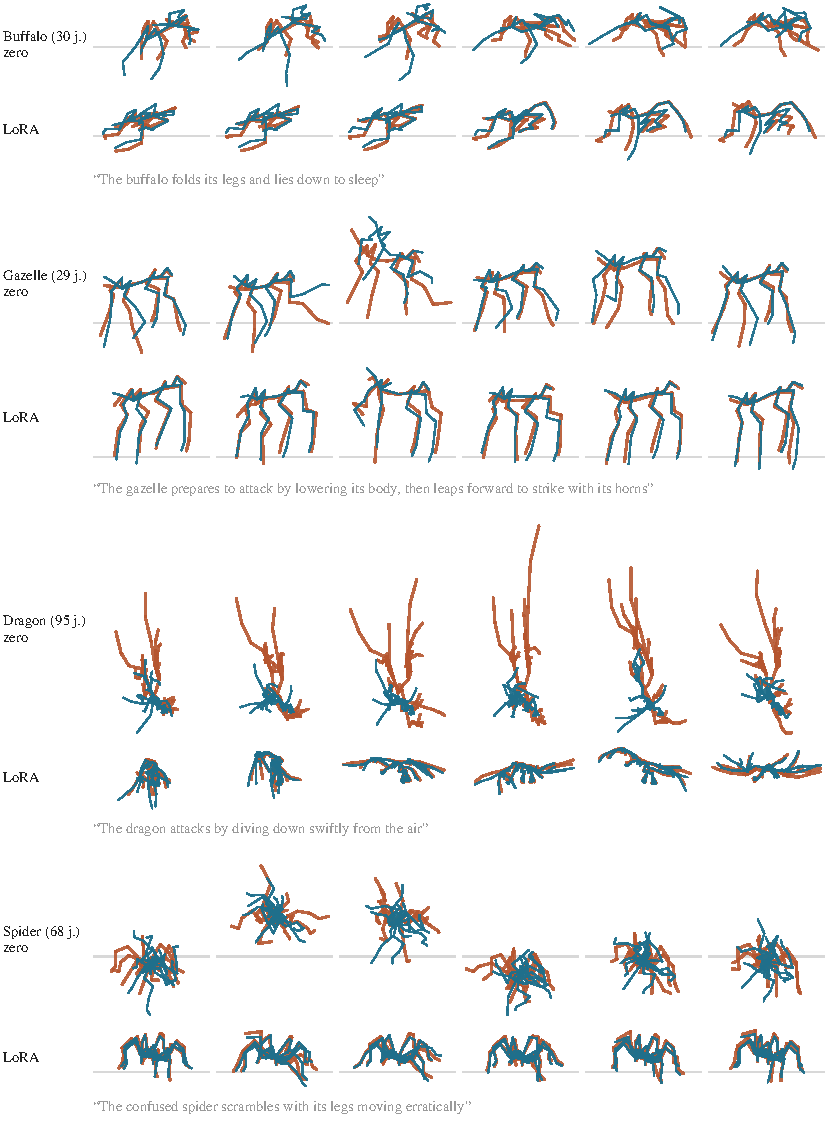
\includegraphics[width=\linewidth]{figures/tb_filmstrips.pdf}
\caption{Truebones arms of Table~\ref{tab:lora}: one held-out clip per rig, six frames spread evenly
over the clip, three-quarter view; the quoted sentence is the conditioning prompt. In every panel the
directly predicted joint positions (clay) are overlaid by the forward kinematics of the predicted
rotations (teal); a visible separation is the projected FK--pose discrepancy (a single view can hide
a disagreement in depth). Rows: the library model with the rig's statistics only (\emph{zero}, the
unadapted snapshot, which is also where the articulation and jitter of that table's zero
column come from; its gap column is read 10 to 15 optimiser steps in) and the per-rig adapter (\emph{LoRA}). Frames are anchored on the root horizontally
and keep their height above the floor; the grey line marks the floor height beneath the root. The
Dragon, a flying rig, is anchored on the root in all axes, which removes its dive trajectory. Both
rows of a rig are drawn at the same scale.}\label{fig:tb_filmstrips}
\end{figure}

\section{A motion demonstration in place of the rest frame}\label{app:demo64}

The demonstration slot of \S\ref{sec:method:model} can hold motion as well as a pose. We trained a
\num{36}M pilot identical to the mainline except that the demonstration is a 64-frame window of
another real clip of the same rig, drawn afresh for every training sample (the grouped objective was
re-calibrated for this condition and returned the same weights, so the two validation losses are on the
same scale). At the same optimiser step (\num{115{,}600}, epoch 200, scored on
the same GPUs) the motion demonstration is worse where the two representations of a pose have to agree
--- validation loss \num{0.270} against \num{0.247} and FK--pose gap \num{0.202} against \num{0.171}
bone lengths --- equal in retrieval (R@1 \num{0.878} for both) and slightly better in FID
(\num{0.010} against \num{0.011}). The attribution of the demonstration pathway is an order of
magnitude smaller than with the rest frame ($3{\times}10^{-4}$ against $5{\times}10^{-3}$), and the
sequence is $26\%$ longer. On the four Truebones rigs of \S\ref{sec:exp:extend} neither condition wins:
zero-training jitter ratios \num{0.95} / \num{6.89} / \num{1.54} / \num{2.94} against the rest frame's
\num{1.92} / \num{6.24} / \num{0.74} / \num{4.71}, and after adaptation \num{0.24} / \num{0.74} /
\num{0.70} / \num{0.17} against \num{0.27} / \num{0.92} / \num{0.62} / \num{0.23}. Because the
demonstration clip is an unrelated motion of the same rig, everything it carries beyond the body plan
is already stated by the caption, and the network learns to ignore it; a moving demonstration also has
to exist at test time, which a rest pose always does. We therefore keep the rest frame.

\section{Validation split}\label{app:split}

The library is split per rig: the rig's clips are sorted by identifier and permuted with one
seeded generator (\texttt{numpy} default generator, seed 0) shared by all rigs in name order, and the
first \num{5}\% of the permutation (at least one clip, none for a rig with a single clip) become
validation, so that every rig with enough clips is represented in both parts. The split is fixed before any model is trained and is shared by
the evaluator and by every generator and adapter in this paper; checkpoints are selected on the
validation loss. Validation holds \num{3{,}899} clips over \num{311} rigs and training
\num{73{,}995} clips. Retrieval pools are formed by chunking the validation set in dataset order
(rigs sorted by name), so a pool of 64 holds clips of one rig or of neighbouring rigs; the last
59 clips do not fill a pool and are excluded from the R-precision but not from the FID or the
matching score.

\paragraph{Shared source animations.} The annotation set exports one source animation to several rigs,
so a motion can appear under more than one clip; retrieval accounts for this in its acceptance sets,
which hold every export of a caption's source motion. On the \num{512} validation clips over
\num{216} rigs whose motion payload and \texttt{(rig, source animation)} pair appear nowhere in
training, the \num{303}M model reaches R@1 \num{0.967} against \num{0.937} on the full validation set
at the same pool size of 32, with the real clips at \num{0.988} and \num{0.975}.

\paragraph{Pool size.} Retrieval among more candidates is harder for the real clips and for the
generated ones alike, and the pool size is a free parameter of the protocol. Table~\ref{tab:pool}
re-scores the same generated samples at four pool sizes; the ranking of the two models does not depend on
the choice, while the gap to the real clips widens with the pool (from \num{0.030} at 16 to \num{0.046} at 128 for
the \num{303}M model); the main text uses 64.

\begin{table}[h]
\centering\small
\caption{R@1 of the same samples (20 steps, $s{=}2$, one seed) re-scored in pools of 16, 32, 64 and
128 formed by chunking the dataset order; the incomplete last pool is dropped. The real clips are scored
by the same evaluator in the same pools.}\label{tab:pool}
\begin{tabular}{lcccc}
\toprule
Pool size & 16 & 32 & 64 & 128 \\
Pools & 243 & 121 & 60 & 30 \\
\midrule
Real clips (reference) & \num{0.985} & \num{0.975} & \num{0.964} & \num{0.961} \\
\method{} (pilot, \num{36}M) & \num{0.938} & \num{0.918} & \num{0.897} & \num{0.891} \\
\method{} (\num{303}M) & \num{0.956} & \num{0.937} & \num{0.922} & \num{0.915} \\
\bottomrule
\end{tabular}
\end{table}


\end{document}
